% ------------------------------------------------------------------------
%
% -------------------      Plantilla_UIS.tex       -----------------------
%
% ------------------------------------------------------------------------
% ------------------------------------------------------------------------
% ------------------------------------------------------------------------
% Versión de plantilla para realización de informes de trabajo de grado
% construida para uso de la Universidad Industrial de Santander.
%
% Reservados todos los derechos
%
% Bucaramanga, Colombia
%
% Febrero 03 de 2019
%
% ------------------------------------------------------------------------
% ------------------------------------------------------------------------
% ------------------------------------------------------------------------
%
% --------------------------\documentclass[letter,oneside,12pt,spanish]{report}

\documentclass[letter,oneside,12pt,spanish]{report}
% ------------------------------------------------------------------------
\usepackage{uislatexstyleAPA} % Libreria UIS APA
% ------------------------------------------------------------------------

% --- AQUÍ VAN TODOS LOS PAQUETES --- %
\usepackage[utf8]{inputenc}
\usepackage{epsfig}
\usepackage{amsmath}
\usepackage{amssymb}
\usepackage{graphicx}
\usepackage{float}
\usepackage{multirow}
\usepackage{wrapfig}
\usepackage{enumitem}
\usepackage{xcolor}
\usepackage{caption}
\usepackage{tcolorbox}
\usepackage{subfigure}
\usepackage{listings}
\usepackage{minted}
\usepackage{csquotes}
\usepackage[style=apa]{biblatex}
\usepackage{geometry}
\usepackage{hyperref}

% --- CONFIGURACIONES DE COLORES --- %
\definecolor{bg}{rgb}{0.95,0.95,0.92}
\definecolor{purple}{rgb}{0.5,0,0.5}
\definecolor{orange}{rgb}{0.9,0.4,0}
\definecolor{codeborder}{RGB}{0,0,0}
\definecolor{codebackground}{RGB}{255,255,255}
\definecolor{codegray}{RGB}{128,128,128}
\definecolor{codegreen}{RGB}{0,153,0}
\definecolor{codeorange}{RGB}{255,125,80}

% --- CONFIGURACIÓN DE LISTINGS --- %
\lstdefinestyle{mystyle}{
	frame=shadowbox,
	backgroundcolor=\color{codebackground},
	commentstyle=\color{codegray},
	keywordstyle=\color{codeorange},
	numberstyle=\tiny\color{codegray},
	stringstyle=\color{codegreen},
	basicstyle=\ttfamily\footnotesize,
	breakatwhitespace=false,
	breaklines=true,
	captionpos=b,
	keepspaces=true,
	numbers=none,
	showspaces=false,
	showstringspaces=false,
	showtabs=false,
	tabsize=2,
	frame=single,
	rulecolor=\color{codeborder},
	framesep=4pt,
	xleftmargin=10pt,
	xrightmargin=10pt,
}
\lstset{style=mystyle}

% --- OTRAS CONFIGURACIONES --- %
\addbibresource{biblio.bib}
\geometry{headheight=15.13202pt}
\captionsetup[figure]{labelfont={bf}, singlelinecheck=false}
\parskip=12pt

\begin{document}                              % Inicio de documento
% ------------------------------------------------------------------------
% Definición silábica de palabras
% ------------------------------------------------------------------------
% \hyphenation{pro-por-cio-nal di-se-ño}
\hypersetup {pdfborder = {0 0 0}}
% ------------------------------------------------------------------------
% Titulo resumido del trabajo que aparecerá en cornisa
% ------------------------------------------------------------------------
\title{AMBIENTE DE APRENDIZAJE PARA LA ENSEÑANZA DE ESTADÍSTICA II}
% ------------------------------------------------------------------------
% Elementos previos al contenido del trabajo
% ------------------------------------------------------------------------ 

\begin{center}

Ambiente de aprendizaje para la enseñanza de Estadística II: un enfoque en teoría, prácticas y autoevaluación\vspace{1.5cm}

Jorge Eduardo Suárez Cortés\\
Daniel Alejandro Sánchez Rodríguez \\ \vspace{1.5cm}

Trabajo de Grado para optar al título de Ingeniero de Sistemas\\ \vspace{1.5cm}

Director\\
Andrés Leonardo González Gómez\\
PhD (c). Ciencias de la Computación\vspace{1.5cm}


Universidad Industrial de Santander\\
Facultad de Ingenierías Fisicomecánicas\\
Escuela de Ingeniería de Sistemas e Informática\\
Ingeniería de Sistemas\\
Bucaramanga\\
2025\\

\end{center}

% Portadilla

\parskip=0pt

\newpage

\titlecontents{paragraph}[0em]{\normalfont\normalsize}{\thecontentslabel. }{}{\titlerule*[1em]{}\contentspage}



\parskip=12pt
\tableofcontents                    

% Tabla de contenido
% ------------------------------------------------------------------------
\newpage

\listoffigures                         % Lista de figuras, tablas y anexos
\newpage
\listoftables
%\listofanexo
% ------------------------------------------------------------------------
\newpage

\chapter*{Glosario}

\begin{description}

\item \textbf{Automatización}: Uso de tecnologías para realizar tareas o procesos sin intervención humana, con el objetivo de aumentar la eficiencia y reducir errores manuales.
\item \textbf{Microsoft Power Platform}: Conjunto de herramientas de Microsoft, que incluye Power Automate, Power Apps y Power BI, que permite la creación de soluciones empresariales con poco o ningún código.
\item \textbf{Python}: Lenguaje de programación utilizado para crear scripts que permiten la conexión, extracción y tratamiento de información de bases de datos.
\item \textbf{RPA (Automatización Robótica de Procesos)}: Tecnología que permite automatizar tareas repetitivas utilizando robots de software.
\item \textbf{SAC (Sistema de Administración Comercial)}: Sistema utilizado para la administración de la información comercial en las empresas.
\item \textbf{JD Edwards}: Sistema de planificación de recursos empresariales (ERP) que gestiona finanzas, proyectos y otros procesos comerciales.
\item \textbf{GUI (Interfaz Gráfica de Usuario)}: Interfaz que permite la interacción del usuario con la solución de software de manera visual e intuitiva, facilitando la recopilación y ejecución de parámetros.


\end{description}


% ------------------------------------------------------------------------
\newpage

% Contenido del Informe
% ------------------------------------------------------------------------
\newpage

\chapter*{Resumen}

\footnotesize{
\begin{description}
  \item[Título:] Ambiente de aprendizaje para la enseñanza de Estadística II: un enfoque en teoría, prácticas y autoevaluación.
  \astfootnote{Trabajo de grado}
  \item[Autores:] Jorge Eduardo Suárez Cortés y Daniel Alejandro Sánchez Rodríguez.
  \asttfootnote{Facultad de Ingenierías Fisicomecánicas. Escuela de Ingeniería de Sistemas e Informática.\\
  	Director: Andrés Leonardo Gonzáles Gómez}
  \item[Palabras Clave:] 
  \item[Descripción:]  
  
  
  
\end{description}}\normalsize

% ------------------------------------------------------------------------

\newpage

\chapter*{Abstract}

\footnotesize{
\begin{description}
  \item[Title:] Learning Environment for the Teaching of Statistics II: A Focus on Theory, Practice, and Self-Assessment.
  \astfootnote{Degree Work}
  \item[Authors:] Jorge Eduardo Suárez Cortés y Daniel Alejandro Sánchez Rodríguez.
  \asttfootnote{Faculty of Physicomechanical Engineering. School of Systems and Computer Engineering.\\
  	Director: Andrés Leonardo Gonzáles Gómez}
  \item[Key words:] 
  \item[Description:] 
  
  
  
  
  

\end{description}}\normalsize

% Abstract

% ------------------------------------------------------------------------
% Capítulos
% ------------------------------------------------------------------------
\newpage

\nnchapter{Introducción}

Este trabajo presenta una propuesta para solventar este problema, que comprende la automatización de la generación de reportes contables, cuya arquitectura integra herramientas de Microsoft Power Platform y Python. Según el trabajo de (\cite{narayn2023building}) donde propone el uso de herramientas de Microsoft Power Platform, donde su integración genera un gran valor añadido a sus capacidades (\cite{narayn2023building}). Microsoft Power Automate ofrece gran facilidad al orquestar flujos de trabajo automatizados (\cite{hvartiainen2024leanmanagement}), el uso de Scripts de Python capaces de hacer conexión a los diferentes orígenes de datos así como su tratamiento (\cite{rattenbury2017principles}), y Microsoft Power Apps para la mejora en la interacción y control del usuario sobre la solución (\cite{psimon2022lowcode}). Se explora la implementación técnica de esta solución, evaluando el impacto de la integración de estas tecnologías por medio del desarrollo de servicios, partiendo de la flexibilidad que ofrece Python a la hora de tratar datos, en la eficiencia operativa de la gestión contable.(\cite{RCore2020})

% ------------------------------------------------------------------------

\newpage


\chapter{Objetivos}

\section{Objetivo General}

\begin{itemize}
    \item Diseñar y desarrollar un entorno virtual para la asignatura de Estadística II, de la Escuela de Ingeniería de Sistemas e Informática de la UIS, que facilite la ejecución de un plan de aula propuesto para la práctica, el aprendizaje y la autoevaluación del contenido de la asignatura, mediante herramientas de Python y R.
\end{itemize}

\section{Objetivos Especificos}

\begin{itemize}
    \item Diseñar un plan de aula modular para la asignatura Estadística II que organice los contenidos teóricos y prácticos en unidades interactivas basadas en Colab Notebooks, Python y R, e incluya calificadores automáticos y ejercicios con retroalimentación instantánea.
    
    \item Implementar un ambiente de aprendizaje virtual en la plataforma Moodle que integre las tecnologías definidas (Colab Notebooks, Python y R) y organice los contenidos teóricos y prácticos junto con materiales didácticos de apoyo, consolidando una experiencia formativa práctica y accesible para la asignatura Estadística II.
    
    \item Establecer instrumentos de medición para las actividades prácticas y autoevaluativas en Moodle (desarrolladas con Python y R), que permitan medir el logro de los resultados de aprendizaje durante el desarrollo del proyecto en el curso de Estadística II.

    \item Pilotear el ambiente virtual de aprendizaje diseñado, con sus contenidos interactivos e instrumentos de evaluación, en por lo menos dos grupos de Estadística II de la Escuela de Ingeniería de Sistemas e Informática de la UIS, con el fin de validar su usabilidad, satisfacción y efectividad en el logro de los resultados de aprendizaje.

\end{itemize}

% ------------------------------------------------------------------------

\newpage

\chapter{Marco Teorico}



%-----------------------------------------------------
\section{Tecnologías implementadas en el proyecto}

\subsection{Node.js y Express.js}

Node.js es un entorno de ejecución basado en el motor V8 de Google Chrome que permite ejecutar JavaScript en el lado del servidor, diseñado bajo un modelo de I/O no bloqueante. Esto lo convierte en una herramienta adecuada para aplicaciones que requieren manejar múltiples solicitudes concurrentes, como plataformas de aprendizaje en línea \parencite{tilkov2010}.

Express.js es un framework minimalista para Node.js que facilita la construcción de APIs y aplicaciones web mediante la organización de rutas, middleware y controladores \parencite{brown2019}. En el proyecto, Node.js y Express.js cumplen el rol de backend principal, gestionando la validación de respuestas de estudiantes, el control de intentos y la comunicación con la base de datos MariaDB.

\subsection{React.js}

React.js es una biblioteca de JavaScript desarrollada por Facebook que permite construir interfaces de usuario basadas en componentes reutilizables \parencite{banks2017}. Su arquitectura con virtual DOM optimiza la actualización de vistas, mejorando la eficiencia y la experiencia de usuario.

El frontend, desarrollado en React.js, centraliza la gestión de calificaciones y el control de intentos de los estudiantes. Su principal ventaja es la transparencia: ante cualquier discrepancia con la calificación calculada por el backend (Node.js), un instructor puede revisar tanto el código enviado por el estudiante como la nota obtenida. Esto facilita una verificación rápida y fundamentada, garantizando la equidad en la evaluación.

\subsection{Bases de datos relacionales (MariaDB)}

MariaDB es un sistema de gestión de bases de datos relacional de código abierto, derivado de MySQL, que organiza los datos en tablas relacionadas bajo el modelo relacional propuesto por \textcite{codd1970}.

Su función en el proyecto es ser el repositorio central de información, donde se almacenan los registros de estudiantes, intentos de ejercicios, calificaciones y respuestas. Gracias a sus características de integridad y consistencia, MariaDB asegura la fiabilidad en el almacenamiento de los resultados generados en los procesos de autoevaluación.

\subsection{Virtualización y contenedores (Docker)}

Docker es una plataforma de contenedores ligeros que empaqueta aplicaciones y dependencias en un entorno aislado, lo que garantiza portabilidad y reproducibilidad \parencite{merkel2014}.

En el proyecto, Docker permite desplegar servicios como el backend, frontend, playit.gg y la base de datos en un entorno controlado, asegurando que las pruebas piloto y los despliegues sean consistentes sin importar el sistema operativo. Su uso facilita la escalabilidad y reduce los problemas de compatibilidad entre entornos de desarrollo y producción.

\subsection{Moodle como LMS}

Moodle es un sistema de gestión de aprendizaje (LMS) de código abierto ampliamente utilizado en la educación superior. Ofrece herramientas para gestionar cursos, usuarios, recursos y actividades de evaluación \parencite{dougiamas2003}.

En este proyecto, Moodle funciona como el entorno de acceso institucional provisto por la UIS, donde los estudiantes encuentran los enlaces a los notebooks de Google Colab, las actividades prácticas y los recursos teóricos. Moodle sirve como el punto de integración pedagógica que articula los recursos tecnológicos desarrollados.

\subsection{Python y R}

Python y R son lenguajes de programación consolidados en el campo del análisis estadístico y la ciencia de datos. Python, gracias a bibliotecas como NumPy, SciPy y Pandas, se ha convertido en una herramienta versátil para la enseñanza y aplicación de métodos estadísticos \parencite{mckinney2017}. R, por su parte, es un lenguaje especializado en estadística y visualización de datos, ampliamente usado en contextos académicos \parencite{rcoreteam2023}.

En el proyecto, para el desarrollo de los graders se emplearán ambos lenguajes de programación, lo que permitirá dotarlos de una mayor versatilidad en su uso.

\subsection{Google Colab}

Google Colab es una plataforma en la nube que permite ejecutar notebooks de Python sin necesidad de instalar software localmente. Combina teoría, código ejecutable y resultados en un único entorno interactivo \parencite{bisong2019}.

Su integración en el proyecto permite a los estudiantes resolver ejercicios en tiempo real, ejecutar simulaciones y enviar sus respuestas al backend para validación. Además, Colab facilita el aprendizaje activo y autónomo.

\subsection{Graders y autoevaluación automatizada}

Los graders son sistemas de evaluación automática que comparan respuestas de estudiantes con soluciones esperadas, otorgando calificaciones y retroalimentación inmediata \parencite{kurnia2001}. Herramientas como nbgrader o Otter-Grader han demostrado su efectividad en la enseñanza de programación y estadística.

En este proyecto, los graders están implementados en el backend desarrollado con Node.js y conectados a los notebooks de Colab. De esta forma, los estudiantes reciben retroalimentación instantánea, lo que fomenta el aprendizaje autónomo y reduce la carga de corrección manual para los docentes.

\subsection{Playit.gg y tunelización de servicios}

Playit.gg es una herramienta que permite crear túneles seguros entre una máquina local y la web pública, facilitando la exposición de servicios locales sin necesidad de configuración compleja de red.

Durante el desarrollo y pruebas piloto del proyecto, Playit.gg se utiliza para exponer el backend y el frontend alojados en contenedores Docker hacia los estudiantes y notebooks de Colab. Esta estrategia permite realizar pilotos de manera controlada.

% ------------------------------------------------------------------------
\newpage


\chapter{Estado del Arte}

\section{Antecedentes}

\noindent La Automatización Robótica de Procesos (RPA, por sus siglas en inglés) ha ganado popularidad en diversas industrias debido a su capacidad para automatizar tareas repetitivas y basadas en reglas, incrementando la eficiencia operativa y reduciendo costos. En el trabajo de (\cite{cooper2019rpa}), se destaca cómo las firmas de contabilidad han adoptado RPA para automatizar la generación de reportes financieros y otras tareas rutinarias, mejorando la precisión y reduciendo los errores humanos. Este tipo de tecnologías permite a las empresas liberar a los empleados de tareas manuales para que puedan enfocarse en actividades de mayor valor añadido.

\noindent Un aspecto clave de la RPA es su capacidad para integrarse sin necesidad de modificar los sistemas subyacentes (\cite{aalst2018bpm}), lo que facilita su implementación en una amplia variedad de entornos empresariales. Sin embargo, como mencionan (\cite{syed2020rpa}), los desafíos actuales incluyen la necesidad de integrar capacidades cognitivas, como el aprendizaje profundo, para mejorar la adaptabilidad de los bots en entornos cambiantes. En este sentido, las plataformas de RPA han comenzado a evolucionar hacia la Automatización de Procesos Inteligentes (IPA, por sus siglas en inglés), que combina RPA con Inteligencia Artificial (IA) y Machine Learning (ML), ofreciendo soluciones más robustas (\cite{gami2019ipa}).

\section{Desarrollo Actual}

\noindent La plataforma Microsoft Power Automate es una herramienta clave en la automatización de procesos de negocios, especialmente en entornos corporativos que ya utilizan la suite de Microsoft 365. Su capacidad para automatizar flujos de trabajo a través de aplicaciones como SharePoint, OneDrive y Outlook permite a las organizaciones integrar datos de múltiples fuentes y realizar tareas complejas sin intervención humana (\cite{microsoft2024powerautomate}). Además, Power Automate ofrece dos tipos principales de automatización: asistida y no asistida. En la automatización asistida, los bots replican acciones humanas en tiempo real, mientras que la automatización no asistida ejecuta tareas programadas sin supervisión (\cite{xerox2023powerautomate}). Esto es particularmente útil para la automatización de procesos contables que requieren la generación y envío de reportes de manera recurrente.

\noindent Python, por su parte, ha sido ampliamente utilizado para la manipulación y tratamiento de datos en procesos de automatización. Herramientas como Pandas y NumPy permiten limpiar, transformar y analizar grandes volúmenes de datos, lo que resulta esencial para asegurar la calidad de los reportes generados automáticamente (\cite{rattenbury2017principles}). Python también ofrece librerías especializadas para la automatización de tareas de escritorio, como `pywinauto` y `pyautogui`, las cuales facilitan la interacción automatizada con aplicaciones en sistemas Windows (\cite{pywinauto2024}). Estas bibliotecas permiten combinar el poder de la automatización robótica con las capacidades de procesamiento de datos de Python, ofreciendo una solución integral para la automatización de procesos contables.

\noindent En empresas como Xerox, Power Automate se ha utilizado para generar reportes de facturación automatizados, eliminando la necesidad de generación manual y reduciendo significativamente los tiempos de procesamiento (\cite{xerox2023powerautomate}). La integración de estas herramientas con tecnologías de Microsoft como Azure Key Vault y SharePoint asegura la seguridad y confiabilidad de los procesos, al utilizar encriptación de 256 bits para la protección de credenciales y datos sensibles.

\noindent En resumen, la Automatización Robótica de Procesos y las plataformas de bajo código como Microsoft Power Automate, combinadas con el poder de Python para el tratamiento de datos, representan una solución robusta y eficaz para la optimización de procesos contables. Estas tecnologías no solo reducen el esfuerzo humano y el riesgo de errores, sino que también mejoran la eficiencia operativa y facilitan el cumplimiento de normativas mediante la automatización de tareas repetitivas y la generación de reportes automáticos.



\newpage

\chapter{Marco de Referencia}
\label{sec:marco-referencia}

\noindent La optimización de procesos es crucial para la competitividad de las organizaciones en el mercado, ya que busca minimizar costos y maximizar el rendimiento, la productividad y la eficiencia. Con el avance de la revolución tecnológica, las empresas han comenzado a implementar la transformación digital para optimizar los procesos en la cadena de valor. Este proyecto está enfocado en el desarrollo de soluciones digitales con el uso de tecnologías de Automatización Robótica de Procesos (RPA), Plataformas de Desarrollo de Bajo Código (LCDPs) y Análisis de Datos (Data Analysis).

\section{Automatización Robótica de Procesos (RPA)}

\noindent La Automatización Robótica de Procesos (RPA) en los últimos años se ha posicionado como una herramienta esencial para la optimización de proceso, debido a paradigmas de automatización de tareas repetitivas en diferentes industrias (\cite{doguc2020rpa}). Su arquitectura es un software que imita las acciones humanas al usar interfaces de usuario de diferentes aplicaciones, permitiendo así una integración sin modificar sistemas subyacentes. En el trabajo de (\cite{doguc2020rpa}) se describe a RPA como una tecnología clave que reduce costos y mejora la eficiencia operativa al automatizar tareas basadas en reglas que anteriormente realizaban los humanos. Esta tecnología no solo aumenta la precisión, sino que también tiene la gran capacidad de liberar a los empleados de tareas manuales, para que se centren en tareas más estratégicas y de mayor valor añadido . Sin embargo, en lo propuesto por (\cite{syed2020rpa}) se analizan los temas contemporáneos y desafíos a los que se enfrenta RPA como nueva tecnología en auge, destacando así la integración de capacidades cognitivas y de aprendizaje profundo. Estos avances no solo permiten a los “bots” ir más allá de la ejecución de tareas repetitivas, sino también la capacidad de adaptarse al entorno cambiante. Por otro lado, menciona la relevancia de la gobernanza centralizada y la preservación del conocimiento del proceso para asegurar la efectividad de RPA. 

\noindent Según (\cite{aalst2018bpm}) el enfoque “de afuera hacia adentro” de RPA lo diferencia de otros métodos de automatización. Este enfoque permite que los sistemas de información existentes permanezcan en el tiempo sin cambios, de la misma manera que los “bots” asumen las tareas humanas. Esto contrasta con enfoques tradicionales como el Procesamiento Directo (STP), que requerían modificaciones en los sistemas subyacentes. En su investigación (\cite{madakam2019rpa}) exploran cómo RPA está transformando la fuerza laboral digital del futuro. La automatización de tareas rutinarias permite que los empleados inviertan su tiempo laboral en actividades que aporten mayor valor añadido a las empresas. Además de esto, se discuten los impactos en la estructura organizacional y la necesidad de gestionar el cambio para asegurar la implementación exitosa de estas tecnologías.

\noindent Finalmente, (\cite{gami2019rpa}) ofrecen una revisión exhaustiva del estado del arte de la implementación de la tecnología RPA y su impacto en las organizaciones empresariales. Destacan los beneficios de su implementación como la reducción de costos y la mejora en la calidad del trabajo, también analizan el encaminamiento de estas tecnologías con dirección a la Automatización de Procesos Inteligentes (IPA), que combina RPA con tecnologías avanzadas como la Inteligencia Artificial (IA) y el Aprendizaje Automático para ofrecer soluciones más robustas y eficaces. 

\noindent La adopción de la Automatización Robótica de Procesos representa una evolución crucial en la manera en que las organizaciones optimizan sus procesos, en aras de la reducción de costo y la mejora constante en la calidad del trabajo. Entre las herramientas de RPA, Microsoft Power Automate se destaca por su capacidad para automatizar flujos de trabajo entra aplicaciones y servicios, permitiendo a las empresas aumentar su eficiencia y productividad mediante la simplificación de tareas diarias.

\noindent El software de automatización Microsoft Power Automate es un servicio de automatización basado en la nube y un conjunto de herramientas de desarrollo de bajo código, diseñado para facilitar la creación de flujos de trabajo automatizados, flujos que a su vez automatizan procesos empresariales. Esta herramienta de bajo código que hace parte de la suite de Microsoft Power Platflorm, tiene como objetivo optimizar las operaciones empresariales al reducir las herramientas manuales y aumenta la eficiencia. Según (\cite{najjar2023powerautomate}) Power Automate facilita la programación autodidacta para usuarios empresariales y no desarrolladores, permitiéndoles construir automatizaciones funcionales si necesidad de conocimientos avanzados de programación. La herramienta soporta varios tipos de automatización, incluyendo flujos en la nube, flujos de escritorio y flujos de procesos de negocio, cada uno adaptado a diferentes necesidades de automatización. Añadido a esto, Power Automate cuenta con más de 400 conectores que permiten integrar servicios como SharePoint, Onedrive, Outlook y Teams, lo que maximiza su utilidad para las organizaciones que ya disponen de herramientas ofrecidas por Microsoft 365.

\noindent En este contexto, (\cite{vartiainen2024leanrpa}) enfatiza cómo Power Automate puede mejorar la experiencia de los empleados mediante RPA. Afirma que la plataforma facilita la automatización de flujos de trabajo completos, integrando datos de diversas fuentes y mejorando la productividad y eficiencia operativa. No solo es útil para automatizar tareas rutinarias, puesto que también es una herramienta poderosa para la integración de datos que mejora la toma de decisiones y la gestión de procesos empresariales. Esta herramienta con su capacidad para manejar flujos en la nube y flujos de escritorio puede adaptarse a una amplia gama de escenarios empresariales, desde la automatización de procesos simples hasta la gestión de flujos de trabajo complejos que involucren múltiples aplicaciones y servicios.

\noindent El asistente virtual interno LUISA de la ESSA, nace de la necesidad de agilizar el acceso a información clave por parte de los trabajadores. Tiene el objetivo de guiar a la Gente ESSA en la resolución de dudas sobre cesantías, vacaciones, reemplazos, pensiones, nómina, permisos, seguridad social y beneficios convencionales. De esta manera mejorar la eficiencia y productividad de los empleados al simplificar la obtención de datos relevantes proporcionando una herramienta integral para la gestión eficaz de temas laborales y prestaciones en todos los niveles y departamentos de la organización. El asistente virtual LUISA está implementado en Microsoft Teams, el cual es un medio de comunicación interno de la empresa. Este asistente virtual fue diseñado con la integración de tecnologías como Microsoft Power Automate, Microsoft Copilot Studio, Microsoft Teams, Microsoft Outlook y Microsoft Excel. (ver Figura \ref{fig:LuisaArquitectura})

\begin{figure}[ht]
    \centering
    \captionof{figure}{ \\ \vspace{0.5cm} Arquitectura LUISA.}
    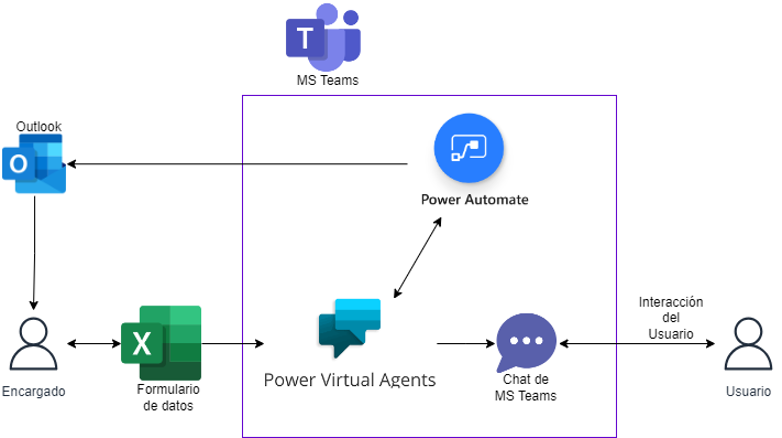
\includegraphics[width=0.7\textwidth]{Figs/arquitectura luisa.png}
    \label{fig:LuisaArquitectura}
    \\Nota: Arquitectura de Luisa, RPA exitoso en la ESSA. León, J. (2024). Diseño propio.
\end{figure}


\noindent La infraestructura de LUISA usa Microsoft Copilot Studio como plataforma principal para diseñar las conversaciones, definir flujos de trabajo y configurar respuestas. Microsoft Teams actúa como el canal de interacción principal, brindando a los usuarios un espacio familiar para acceder a las capacidades del asistente virtual de manera eficiente. En la integración con Microsoft Power Automate usa palabras desencadenadoras, las cuales al ser accionadas accionan un flujo creado previamente el cual tomará una serie de respuestas o acciones de envío de correos para dar soluciones al usuario. La estructura de los temas hallados en LUISA (ver Figura \ref{fig:LuisaEstructura}). está ramificado según el sindicato, pues el tipo de solicitud y sus respuestas son diferentes en cada una. 

\begin{figure}[ht]
    \centering
    \captionof{figure}{ \\ \vspace{0.5cm} Estructura LUISA.}
    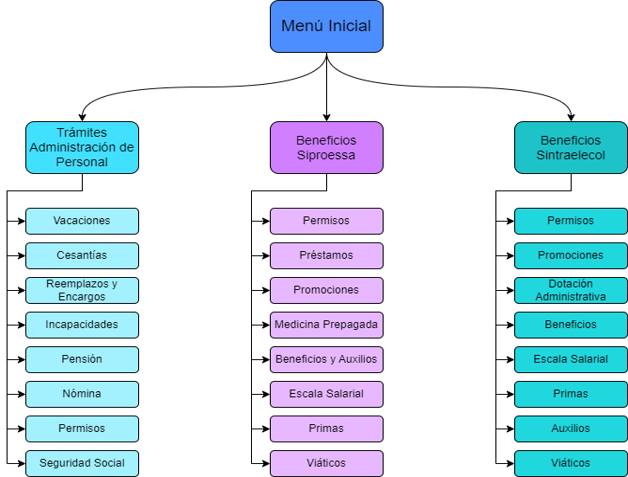
\includegraphics[width=0.7\textwidth]{Figs/estructura luisa.png}
    \label{fig:LuisaEstructura}
    \\Nota: Estructura de Luisa, RPA exitoso en la ESSA. León, J. (2024). Diseño propio.
\end{figure}


\section{Plataformas de Desarrollo de Bajo Código (LCDP's)}

\noindent Las plataformas de desarrollo de bajo código (LCDPs) han emergido como una solución innovadora para enfrentar la creciente demanda de aplicaciones. En el trabajo de (\cite{alsaadi2021lcdp}) se indica que las LCDPs permiten a las organizaciones crear aplicaciones rápida y fácilmente por medio de interfaces visuales y componente preconstruidos, disminuyendo significativamente la necesidad de codificación manual. Este enfoque libera el desarrollo de software, pues permite a empleados participar en desarrollos de aplicaciones sin tener un estudio técnico avanzado previo, a ellos se les conoce como desarrolladores ciudadanos. En consecuencia, (\cite{prinz2021lcdp}) destacan el aumento en la relevancia de las LCDP y cómo están transformando las operaciones y la estructura organizativa al agilizar el desarrollo, consecuente a esto la reducción de los costos asociados a la contratación y formación de personal en el cargo de desarrolladores especializados.

\noindent Las LCDPs ofrecen varios beneficios importantes para las empresas, (\cite{sharma2023appsmith}) indican que entre estos beneficios se encuentran la rapidez y eficiencia en el desarrollo, lo que permite desplegar aplicaciones en tiempos verdaderamente despreciables comparándolos con métodos que se realizaban anteriormente. Además, la facilidad de integración con diferentes orígenes de datos y sistemas, mejorando así la cooperación operativa en las organizaciones. No obstante, Käss, Strahringer y Westner et al. (2023) afirman que la accesibilidad y facilidad de uso de estas plataformas permiten a los desarrolladores ciudadanos crear soluciones personalizadas que atienden necesidades específicas del negocio, promoviendo una mayor innovación interna. Sin embargo, la adopción de LCDP también enfrenta desafíos. 

\noindent Finalmente, (\cite{alsaadi2021lcdp}) mencionan la necesidad establecer estructuras claras de gobernanza y medidas de seguridad robustas para así garantizas en gran parte la calidad y protección de los datos.

\noindent En conclusión, las plataformas de desarrollo de bajo código están reestructurando el entorno del desarrollo de software empresarial, permitiendo a las organizaciones generar más agilidad e innovación en su cadena de valor. El aumento de la inclusión de estas plataformas en las empresas trae consigo la necesidad de implementar procesos de gobernanza y seguridad en aras de la maximización de su potencial. Una de las herramientas más relevantes en este contexto es Microsoft Power Apps, pues ofrece una robusta plataforma de bajo código, lo cual permite a los usuarios empresariales no solo desarrollar aplicaciones rápidamente, sino también integrar soluciones en su ecosistema.

\noindent La herramienta Microsoft Power Apps no deja de revolucionar cada vez más el desarrollo de aplicaciones por medio de su plataforma de bajo código, la cual permite a los usuarios crear aplicaciones empresariales sin la necesidad de conocimientos avanzados en programación por parte de los empleados. Según (\cite{pandit2024lcdp}), Power Apps destaca en el contexto de LCDPs por su interfaz intuitiva la cual se trata de arrastrar y soltar, sus conectores preconstruidos y plantilla, y su gran capacidad de integración con diversas fuentes de datos. Esta plataforma no solo facilita a los usuarios la creación rápida de aplicaciones personalizadas, sino que también se destaca por fomentar la innovación tecnológica dentro de las organizaciones. En este sentido (\cite{narayn2023modernworkplace}) destaca la importancia de Power Apps en el entorno del trabajo moderno, integrándolo con herramientas como SharePoint Online, Power Automate y Microsoft Teams para con ello ofrecer soluciones completas de colaboración y gestión de contenido. Por otro lado, (\cite{diRuscio2022lcdp}) subraya cómo esta plataforma, en combinación con la ingeniería dirigida de modelos (MDE), proporciona un enfoque eficiente y flexible para el desarrollo de software, abordando tanto los aspectos técnicos como organizativos de la creación de aplicaciones.

\noindent La Universidad McGill es un notable caso de éxito en su implementación de Microsoft Power Apps y Microsoft Teams, para el desarrollo de una plataforma educativa virtual de la disciplina patología. Este caso ha sido descrito por (\cite{rajaram2022pathology}). El departamento de Patología Universidad McGill en respuesta a la pandemia de COVID-19, implementó Microsoft Power Apps y Microsoft Teams (ver Figura \ref{fig:McGuill}) para continuar la educación de los estudiantes de manera remota. Esta plataforma personalizada permitió a los residentes acceder a imágenes digitalizadas de diapositivas completas, participar en sesiones educativas y realizar exámenes a distancia (ver Figura \ref{fig:McGuillAPP}).


\begin{figure}[ht]
    \centering
    \captionof{figure}{ \\ \vspace{0.5cm} Plataforma virtual Universidad McGuill.}
    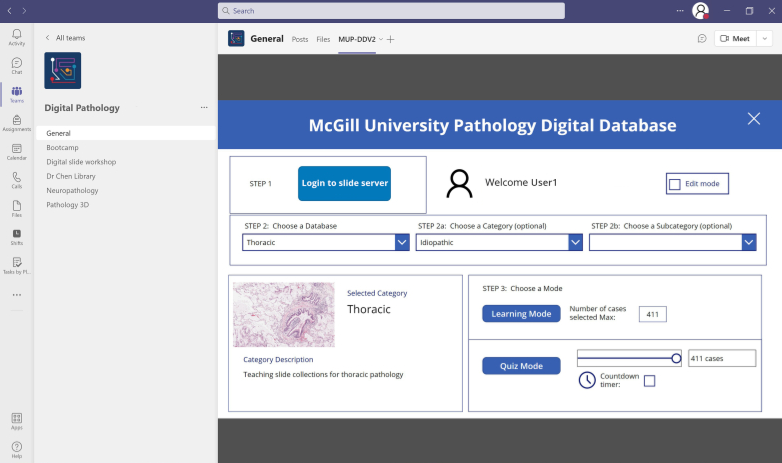
\includegraphics[width=0.7\textwidth]{Figs/mcgill university.png}
    \label{fig:McGuill}
    \\Nota: Visión de la aplicación Patología Digital. \cite{rajaram2022pathology}. Adaptación.
\end{figure}



\noindent La integración con Microsoft Teams facilitó la organización y el acceso a todos los recursos educativos, mejorando así significativamente la continuidad y calidad de la educación durante esta etapa. Esta implementación demuestra el éxito de Power Apps, y cómo puede ser usado para desarrollar soluciones educativas innovadoras y eficiente, incluso fuera de este contexto. La gran capacidad de adaptación a las necesidades cambiantes y con ello asegurando la continuidad educativa en tiempos de crisis.


\begin{figure}[ht]
    \centering
    \captionof{figure}{ \\ \vspace{0.5cm} Plataforma virtual Universidad McGuill.}
    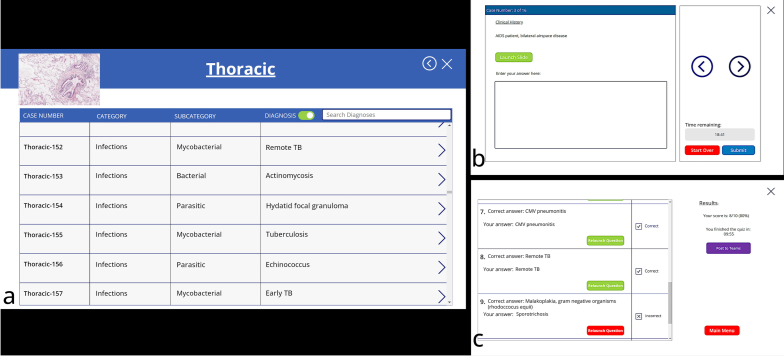
\includegraphics[width=0.7\textwidth]{Figs/mcgill university aplication.png}
    \label{fig:McGuillAPP}
    \\Nota: Aplicación de Patología digital que muestra: a) Lista de imágenes de portaobjetos completos con sus diagnósticos   que se pueden lanzar. b) Modo de cuestionario dentro de la aplicación. c) Visualización de las respuestas evaluadas por los usuarios. \cite{rajaram2022pathology}. Adaptación.
\end{figure}



\section{Tratamiento de datos (Data Wrangling)}

\noindent El proceso de limpieza al que se someten los datos, conocido como Data Wrangling, es parte importante en el ciclo de vida de los datos, puesto que este proceso asegura que los conjuntos de datos sean precisos, consistentes y compactos, esto los vuelve utilizables. Según (\cite{rattenbury2017principles}) la identificación y corrección de errores, la eliminación de duplicados y el tratamiento de valores atípicos y faltantes, es lo que implica este proceso. No obstante, (\cite{kazil2016data}) aseguran que la implementación efectiva permite que los análisis se basen en datos confiables, lo cual es crucial para obtener resultados significativos en su utilización. Las técnicas más utilizadas en el Data Wrangling son la atribución de valores faltantes, la normalización de datos numéricos, y la codificación de variables categóricas. Estas técnicas ayudan a mejorar la calidad de los datos, asegurando decisiones empresariales basadas en estos datos cohesionados, sean precisas y confiables.

\noindent En este contexto, Python es una de las herramientas más usadas en la limpieza de datos debido a su versatilidad y robustez del compendio de bibliotecas. Herramientas como Pandas, NumPy tienen una colección de funciones avanzadas que permiten la manipulación y transformación de los datos, consiguiendo facilitar tareas como la eliminación de duplicados, la gestión de valores faltantes, irregularidades en los registros y normalización de características numéricas (\cite{vanderAalst2018rpa}) , (\cite{jafari2024datapreprocessing}). La biblioteca Pandas, permite la lectura, transformación y limpieza de grandes conjuntos de datos, que hace llamar “DataFrame”, de manera eficiente, lo cual es parte fundamental para la preparación de los datos a análisis con mayor complejidad y modelado predictivo (\cite{provost2013datascience}). Además, Python es un lenguaje de programación con facilidad de uso, y su comunidad de usuarios la hacen la opción más accesible con un sector objetivo de oscila entre principiantes y profesionales experimentados en ciencia de datos. En conclusión, el uso de Python no solo optimiza el proceso de cleaning, sino que también ofrecen una base sólida para realizar análisis de datos más profundos y precisos. 


\section{Seguridad}

\noindent En el contexto de las soluciones digitales, la seguridad en la protección de datos y credenciales es primordial. Por ello, aquellos trabajos que pretenden manejar información sensible deben implementar mecanismos sólidos de seguridad para evitar brechas que expongas información con alto riesgo, como credenciales o incluso información de terceros involucrados. Teniendo en cuenta esto, existen diversas herramientas y tecnologías cuyas características de seguridad integradas permiten la gestión y protección de la información durante su ciclo de vida útil. Algunos métodos de estos son:

\subsection{Encriptación de Datos Sensibles}

\noindent Uno de los más importantes métodos para proteger los datos sensibles, es la encriptación de estos. La encriptación simétrica, especialmente mediante el algoritmo AES-256, se ha consolidado como uno de los métodos más seguros y eficientes para proteger datos en reposo. Este tipo de encriptación utiliza una única clave para cifrar y descifrar la información, garantizando así que solo se pueda acceder a los datos protegidos por medio de autorización. Los archivos de configuración, como aquellos que contienen credenciales de acceso a bases de datos, deben ser cifrados antes de ser almacenados para protegerse de accesos no autorizados (\cite{cryptography2024fernet}).

\noindent Un punto importante parte de la necesidad de que la clave de encriptación debe estar gestionada de manera correcta, evitando que sea vulnerada. Existen herramientas de gestión de secretos como Azure Key Vault, que gestiona claves en entornos locales. Estas herramientas permiten almacenar y tener control sobre el acceso a estas claves de manera segura (\cite{microsoft2024keyvault}).

\subsection{Conexiones Seguras a Bases de Datos}

\noindent En proyectos que dependen de consultas y operaciones sobre bases de datos, establecer conexiones seguras es crucial para proteger la información durante su transmisión. Bases de datos comerciales, como Oracle y SQL Server, ofrecen soporte para conexiones cifradas a través de protocolos SSL/TLS. Estos protocolos garantizan que los datos se transmitan de forma segura, evitando que sean interceptados o modificados por terceros no autorizados.

\noindent En la práctica, el uso de la librería Python-oracledb en modo Thick, por ejemplo, facilita la configuración de conexiones seguras entre la solución y la fuente de datos, aprovechando las librerías cliente de Oracle para implementar Capa de Sockets Seguros/Seguridad de la capa de transporte (SSL/TLS) (\cite{oracle2024python}). Este proceso asegura el tránsito de información entre el servidor y las bases de datos, para solidificar aún más la solución, algunos trabajos refuerzan la seguridad haciendo uso de redes privadas virtuales (VPN) y firewalls para restringir el acceso a la base de datos únicamente a usuarios y direcciones IP autorizadas, brindando una capa adicional de seguridad (\cite{microsoft2024vpn}).

\subsection{Seguridad en la plataforma Microsoft Power Platform}

\noindent Microsoft Power Platform, que incluye herramientas como Power Apps y Power Automate, contiene prácticas de seguridad integradas para controlar los accesos a las soluciones creadas y garantizar la protección de los datos usados en los entornos. La plataforma implementa un modelo de control de acceso basado en roles (RBAC), que permite asignar permisos específicos a los usuarios en función de su rol. Esta segmentación asegura que solo los usuarios autorizados puedan acceder y manipular aplicaciones, flujos o datos sensibles dentro del entorno (\cite{microsoft2024securityroles}).

\noindent Adicional a esto, contiene capacidades de cifrado de datos en tránsito y en reposo, utilizando protocolos como TLS para la transmisión de información y AES-256 para el almacenamiento de datos sensibles (\cite{microsoft2024encryption}). Garantizando que las conexiones y los datos almacenados en la nube estén protegidos de accesos no autorizados y manipulaciones.

\noindent Basándonos en esta base conceptual, se debe profundizar en la metodología de investigación.

% ------------------------------------------------------------------------

\newpage

\chapter{Metodología}

\noindent En esta sección se aborda de qué manera se van a llevar a cabo los objetivos planteados inicialmente, en la cual se notarán las configuraciones que se deben realizar en los softwares, las tecnologías que se van a usar, y qué se va a realizar con ellas. Consta de 4 etapas, las cuales son la conexión a las bases de datos y extracción de la información por medio de Python, la automatización de este proceso con Power Automate, la realización de la GUI con PowerApps y finalmente, la implementación de pruebas, documentación y manuales técnicos y de soporte. 


\section{Script de Python}

\noindent Se propone crear un script mediante el cual se utiliza la librería de Python para conectar con las bases de datos usadas en los sistemas de información. Estas bases de datos están alojadas en Oracle, por lo que se requiere llevar a cabo la conexión a través de la librería \texttt{Python-oracledb}. Esta librería, en particular, tiene dos modos de conexión: la arquitectura del modo "Thin" (ver Figura \ref{fig:modothini}) permite la conexión directa a la base de datos, la cual puede estar en la misma máquina o puede ser remota (\cite{oracle2024python}).


\begin{figure}[ht]
    \centering
    \captionof{figure}{ \\ \vspace{0.3cm} Modo Thin.}
    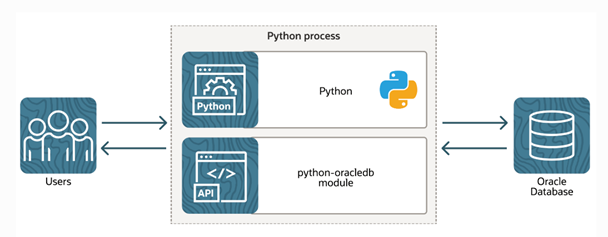
\includegraphics[width=0.6\textwidth]{Figs/modo thin.png}
    \label{fig:modothini}
    \\Nota:Arquitectura del controlador python-oracledb en modo Thin. (\cite{oracle2024python}). Adaptación.
\end{figure}

\begin{figure}[ht]
    \centering
    \captionof{figure}{ \\ \vspace{0.3cm} Modo Thick.}
    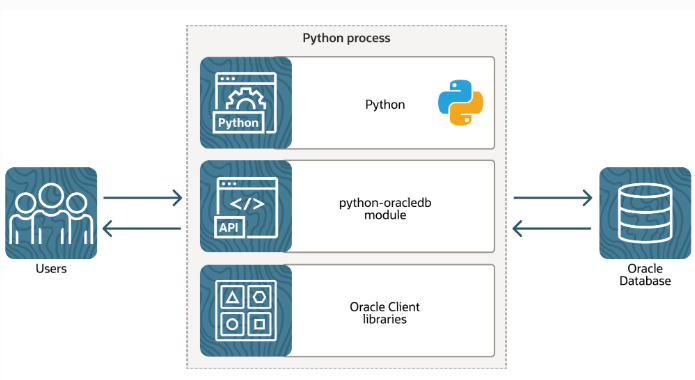
\includegraphics[width=0.6\textwidth]{Figs/modo thick.png}
    \label{fig:modothick}
    \\Nota:  Arquitectura del controlador Python-oracledb en modo Thick. (\cite{oracle2024python}). Adaptación.
\end{figure}



\noindent El otro modo es el “Thick” (ver Figura \ref{fig:modothick}). Python-oracledb opera en este modo cuando se enlaza con las librerías de Oracle Client, lo que le proporciona funcionalidad adicional. Dado que las bases de datos con las que se requiere establecer la conexión son de versiones antiguas, se propone utilizar Python-oracledb en modo Thick para garantizar compatibilidad y aprovechar sus capacidades avanzadas (\cite{oracle2024python}).


\noindent Posterior a la conexión, se hace una consulta a la base de datos, por medio de un query, normalmente está hospedado en un archivo con formato sql, esta consulta va a traer aquella información que se especifique, y para mayor facilidad en el siguiente proceso, se convertirá a un formato DataFrame (ver Figura \ref{fig:pandas}). Este formato permite a la librería Pandas de Python limpiar y procesar la información con todas las herramientas que posee. Hay que hacer procesos de limpieza: eliminar duplicados, eliminar nulos, cruzar información con archivos de Excel, cambiar los valores de una columna en específico y cambiar el tipo de dato para operarlo con otros. Esta librería permite obtener un reporte con el formato establecido, y el tipo de archivo necesario (.txt) (\cite{pandas2024}).

\begin{figure}[ht]
    \centering
    \captionof{figure}{ \\ \vspace{0.5cm} DataFrame \texttt{Pandas}.}
    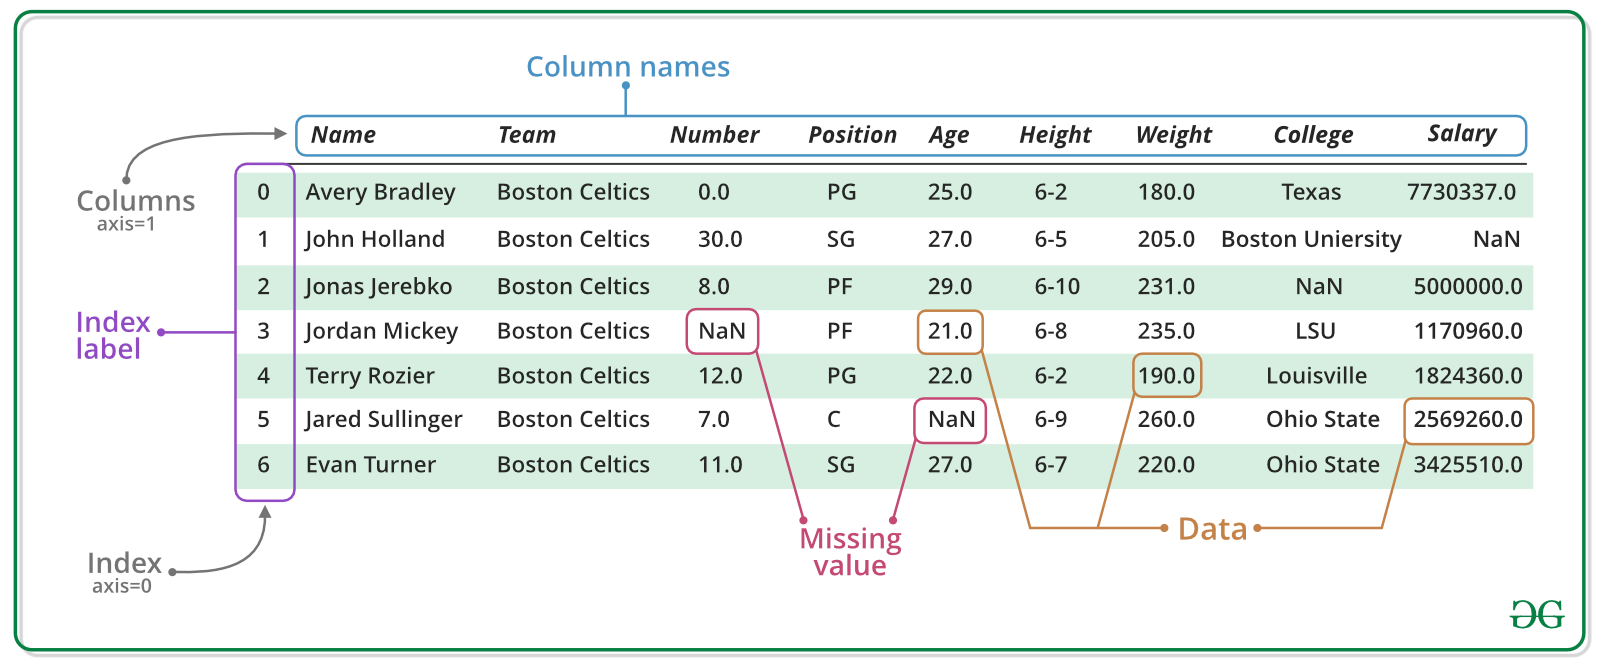
\includegraphics[width=0.7\textwidth]{Figs/pandas.png}
    \label{fig:pandas}
    \\Nota:  Estructura de un DataFrame de Pandas. (\cite{pandas2024}). Adaptación.
\end{figure}



\noindent Finalmente, este Script de Python resulta en un archivo plano que contiene la información lista para reportar.


\section{Automatización Robótica de Procesos}

\noindent Como consiguiente de este proceso, alguien debe tener la responsabilidad de ejecutar este Script, y aquí se introduce el papel de la Automatización Robótica de Procesos (RPA) por medio de la herramienta Microsoft Power Automate, se crean flujos de nube, cuyo desencadenador es la captura de parámetros por medio de una interfaz. A partir de esto, la herramienta low-code proporciona gran facilidad para la creación de los flujos, para este caso en particular se requiere crear un flujo que ejecute el Script de Python por medio de Power Automate Desktop (ver Figura \ref{fig:runscript}). Este flujo pondrá los parámetros capturados en el momento que se desencadena, y los pondrá en el Script, para seguir con la ejecución de este, ya que este Script da como resultado un archivo plano, el siguiente flujo buscará este archivo plano en la ruta donde se hospedó, para cargarlo en la página web requerida, para ello tendrá que validar con el usuario, por ello enviará un flujo de aprobación (\cite{stackoverflow2024pythonpowerautomate}).


\begin{figure}[ht]
    \centering
    \captionof{figure}{ \\ \vspace{0.5cm} Ejecución Script con Power Automate}
    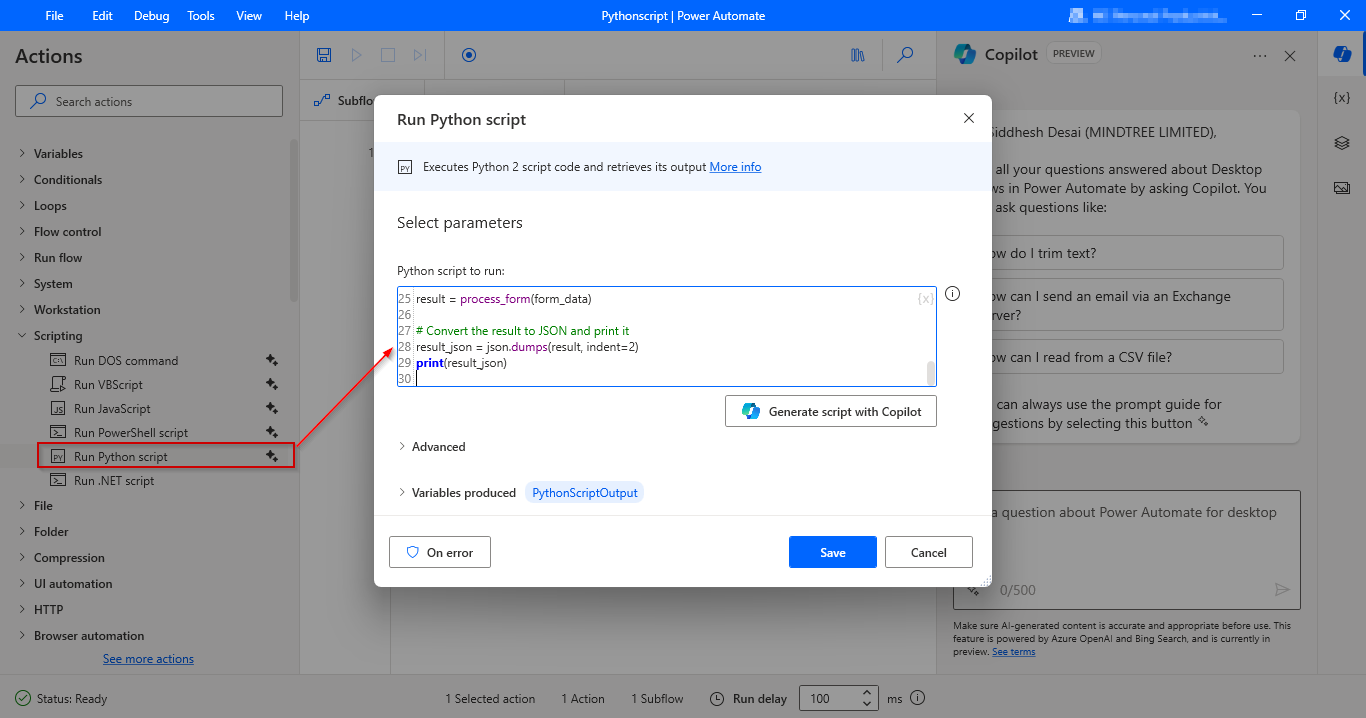
\includegraphics[width=0.7\textwidth]{Figs/ejecicion script - metodologia.png}
    \label{fig:runscript}
    \\Nota:  Ejemplo de la ejecución de un Script de Python desde un flujo de Power Automate Desktop. (\cite{stackoverflow2024pythonpowerautomate}). Adaptación.
\end{figure}

\noindent Siendo la aprobación efectiva, se construye el flujo que carga la información, por lo que irá a obtener las credenciales en un archivo cuya ruta conoce y hará el respectivo cargue. Una vez hecho lo anterior, se enviará un correo masivo a las entidades por medio de Outlook, este se enviará mediante un conector de Power Automate, cuyo contenido incluirá una tabla HTML dinámica, reflejando la información reportada a cada entidad.

\noindent Siendo la aprobación efectiva, se construye el flujo que carga la información, entonces irá a obtener las credenciales en un archivo cuya ruta conoce, y hará el respectivo cargue. Hubo hecho lo anterior, este enviará un correo masivo a las entidades por medio de Outlook, este es un conector de Power Automate, cuyo contenido tendrá una tabla HTML dinámica, reflejando la información reportada a cada entidad. 

\section{Interfaz Gráfica de Usuario}

\noindent Para finalizar el desarrollo, los parámetros necesarios para la creación y cargue del reporte, se deben capturar por medio de una interfaz gráfica de usuario (GUI), para ello se utiliza la herramienta de Microsoft, Power Apps. Gracias a la facilidad que esta herramienta presta para la creación de interfaces se propone crear una de manera que sea un formulario (ver Figura \ref{fig:createapp}) (\cite{tapanm2024powerapps}). Este formulario dará la posibilidad al usuario de digitar los parámetros requeridos para el reporte, y un botón cuya funcionalidad será ser el desencadenador de los flujos posteriores a estos, los cuales mantienen la lógica del proceso (ver Figura \ref{fig:button}) (\cite{tapanm2024powerapps}).

\begin{figure}[ht]
    \centering
    \captionof{figure}{ \\ \vspace{0.5cm} Ejemplo Form Power Apps }
    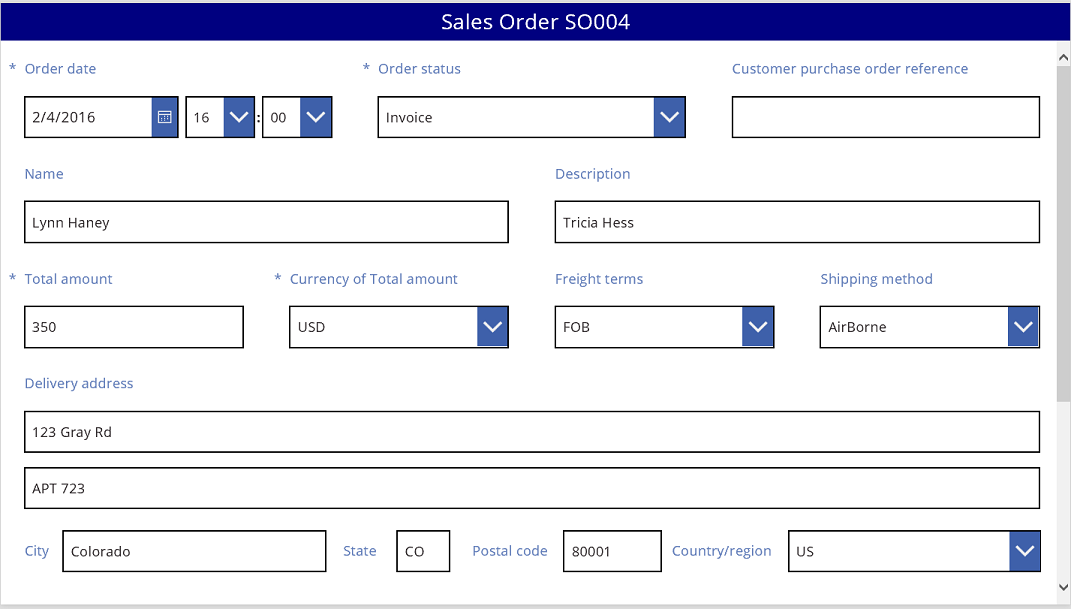
\includegraphics[width=0.7\textwidth]{Figs/creacion app ejemplo.png}
    \label{fig:createapp}
    \\Nota:  Ejemplo de la creación de un formulario para la captura de parámetros en Power Apps (\cite{tapanm2024powerapps}). Adaptación.
\end{figure}

\begin{figure}[ht]
    \centering
    \captionof{figure}{ \\ \vspace{0.5cm} Botón que ejecuta un flujo}
    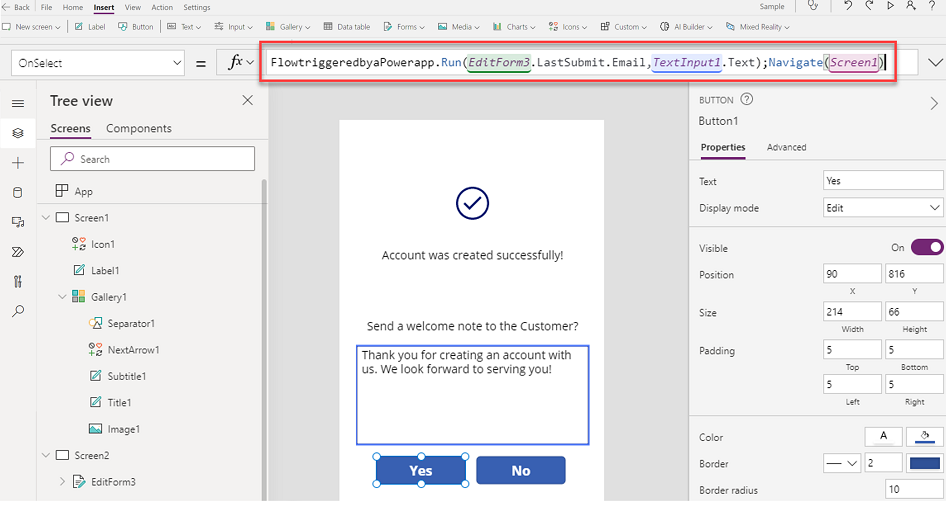
\includegraphics[width=0.7\textwidth]{Figs/boton que ejecuta flujo.png}
    \label{fig:button}
    \\Nota:  Ejemplo de la configuración de un botón como desencadenador de un flujo de Power Automate (\cite{tapanm2024powerapps}). Adaptación.
\end{figure}

\section{Implementación de seguridad}


\noindent Con el fin de proporcionar una seguridad eficiente al proyecto y proteger tanto las credenciales como las conexiones entre la máquia y las bases de datos, se investigó las capacidades de seguridad proporcionadas por Microsoft Power Platform y la implementación de encriptación de credenciales mediante librería en Python. 

\subsection{Roles y Permisos en Microsoft Power Platform}

\noindent Microsoft Power Platform utiliza un sistema de roles basado en permisos que indica qué acciones puede realizar un usuario en cada entorno (\cite{microsoft2024environments}). Los entornos son creados para fines de desarrollo, pruebas o producción (Ver Figura \ref{fig:entornos}). Estos roles se dividen en 3 principales categorías:

\subsubsection{Administrador de entorno}

\noindent Este rol tiene acceso completo al entorno, lo que incluye capacidad para gestionar usuario, flujos, aplicaciones e incluso configuraciones de seguridad.

\subsubsection{Creador de aplicaciones}

\noindent Un creador de aplicaciones puede crear y personalizar aplicaciones en el entorno, pero su capacidad, pero su alcance en otros aspectos del entorno es limitado.

\subsubsection{Usuario básico}

\noindent Tienen permisos restringidos y solo pueden utilizar las aplicaciones y flujos a los que se les haya otorgado acceso, un administrador de entorno.

\begin{figure}[ht]
    \centering
    \captionof{figure}{ \\ \vspace{0.5cm} Gestión de entornos en Power Platform }
    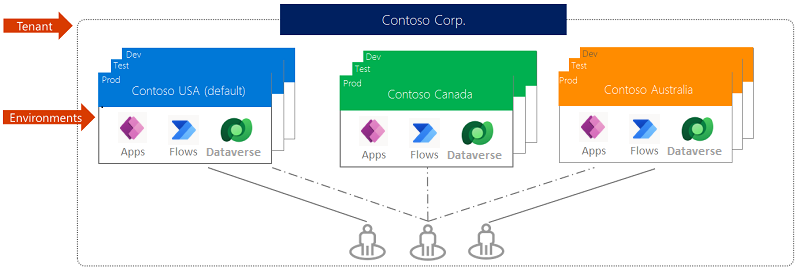
\includegraphics[width=0.7\textwidth]{Figs/gestion de entornos microsoft.png}
    \label{fig:entornos}
    \\Nota:  Implementación de seguridad por medio de entornos administrados en Power Platform (\cite{microsoft2024environments}). Adaptación.
\end{figure}


\subsection{Conexión de Servicios}

\noindent La comunicación entre los servicios de Microsoft, como Power Automate, Power Apps, Outlook o Sharepoint está protegida por medio de cifrado de datos en tránsito (TLS) (Ver Figura \ref{fig:tls}) y datos en reposo (AES-256), garantizando así que la información se mantenga protegida frente a accesos no autorizados en la transmisión y almacenamiento de esta (\cite{microsoft2024encryption}).

\noindent Por ello, es vital configurar de manera correcta los roles de los usuarios, con el fin de evitar la exposición no deseada de datos sensibles. En entorno de desarrollo y pruebas, es común tener un mayor acceso, pero en entornos de producción es recomendable restringir los permisos solo a usuarios esenciales (\cite{microsoft2024environments}).

\begin{figure}[ht]
    \centering
    \captionof{figure}{ \\ \vspace{0.5cm} Cifrado de datos en Power Platform}
    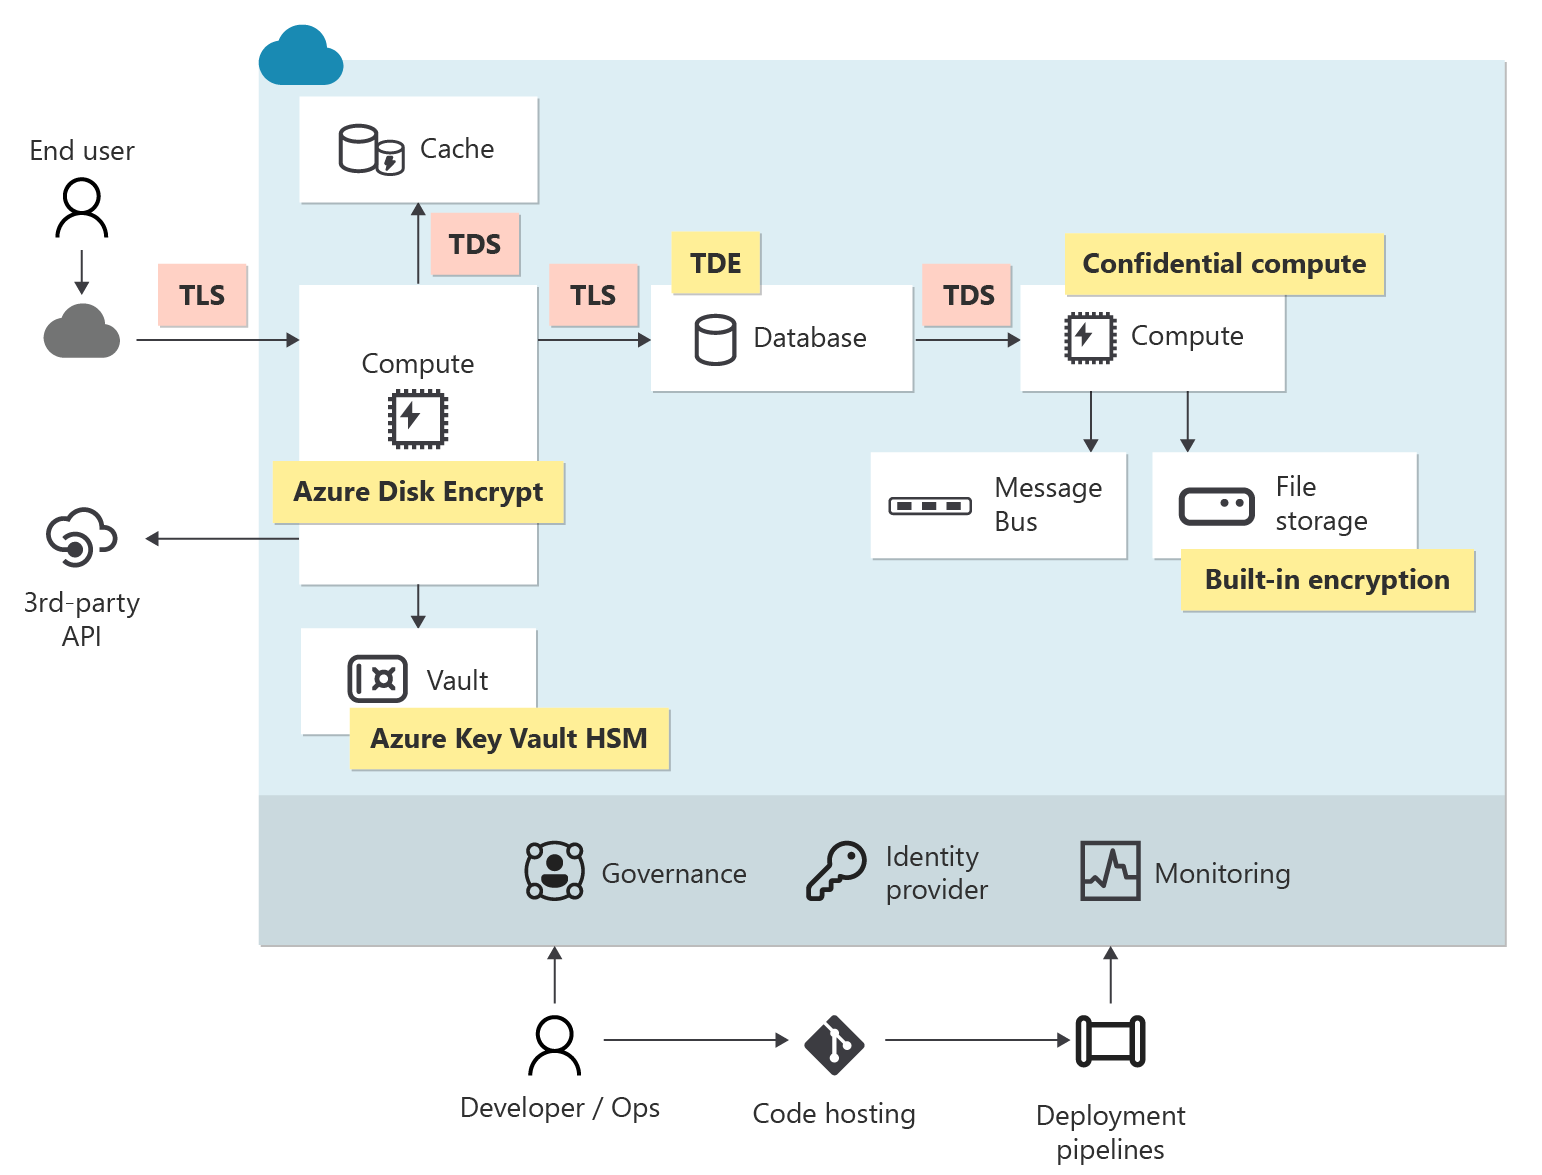
\includegraphics[width=0.7\textwidth]{Figs/TLS.png}
    \label{fig:tls}
    \\Nota:  Cifrado de datos en tránsito (TLS) usado por Microsoft Power Platform (\cite{microsoft2024encryption}). Adaptación.
\end{figure}


\subsection{Encriptación de credenciales}

\noindent Para asegurar las credenciales de acceso a las bases de datos como SAC o JD Edwards, se propone un sistema de encriptación basado en Python que utiliza cifrado simétrico (AES-256) a través de la biblioteca cryptography (Ver Figura \ref{fig:fernet}). Este enfoque asegura que las credenciales se almacenen en un archivo JSON encriptado, y que únicamente sean desencriptadas durante la ejecución del Script (\cite{microsoft2023securitygovernance}).

\subsubsection{Generación de clave}

\noindent Una clave de encriptación se genera una única vez y se almacena en un archivo protegido (\cite{microsoft2023securitygovernance}).

\subsubsection{Almacenamiento seguro}

\noindent El archivo que contiene la clave, debe ser guardado en una ubicación segura, cuya autorización será restringida para su acceso (\cite{microsoft2023securitygovernance}).

\subsubsection{Encriptación de credenciales}

\noindent Durante el desarrollo del proyecto, las credenciales se encriptan usando esta clave previamente gestionada y se almacenan en un archivo JSON encriptado (\cite{microsoft2023securitygovernance}) y (\cite{python2024cryptography}).

\subsubsection{Desencriptación}
\noindent Cuando se ejecuta el módulo del Script que requiere las credenciales, el archivo de claves es utilizado para desencriptar el contenido del archivo JSON (\cite{microsoft2023securitygovernance}) y (\cite{python2024cryptography}).


\noindent Es fundamental que el archivo de claves esté protegido con permisos adecuados. Solo el servidor que ejecuta el Script debe tener acceso a estos archivos, lo cual puede gestionarse mediante permisos del sistema de archivos o almacenamiento de secretos locales (\cite{oracle2024pythondriver}).

\noindent Como alternativa, se propone el uso de variables de entorno con el fin de gestionar la clave de encriptación evitando almacenar la clave en un archivo. Esto reduce los riesgos de exposición en sistemas compartidos. Las variables de entorno se configuran al nivel del sistema operativo, de modo que las claves nunca se almacenan directamente en los archivos de código (\cite{microsoft2024apikeys}).


\begin{figure}[ht]
    \centering
    \captionof{figure}{ \\ \vspace{0.5cm} Encriptación Simétrica}
    
\includegraphics[width=0.7\textwidth]{Figs/encriptacion simetrica.png}
    \label{fig:fernet}
    \\Nota:   Encriptación simétrica usada por la librería Criptography Fernet (\cite{cryptography2024fernet}). Adaptación.
\end{figure}


\subsection{Conexión entre máquinas}

\noindent Con el fin de garantizar la seguridad de la conexión entre el servidor donde será hospedada la solución y las bases de datos (SAC y JD Edwards) como se definió anteriormente, el uso de la librería Python-oracledb en modo Thick que soporta el protocolo SSL/TLS para el cifrado de las conexiones (\cite{microsoft2024keyvault}).

\noindent Debido a que la solución será desplegada en un entorno corporativo, el cual usa redes privadas virtuales (VPN) o túneles seguros para la conexión a bases de datos, especialmente en entornos remotos. Y el uso de firewalls para limitar qué IPs pueden acceder a la base de datos, consolidad la seguridad eficiente de la conexión (\cite{owasp2024cryptographic}) y (\cite{realpython2024secrets}).



\section{Pruebas y Conclusiones}

\noindent Finalmente, teniendo la estructura planteada, se harán pruebas funcionales, verificando información con reportes contraídos y cargados anteriormente, atrapando excepciones y posibles errores que los flujos, o el Script puedan presentar, esto con el fin de que el mantenimiento de esta solución a futuro sea simple. Teniendo un testeo perfecto, se propone buscar técnicas para obtener un despliegue eficaz junto con la estabilización del proyecto en producción, dando lugar al usuario generar los reportes y sus respectivas verificaciones. Como trayecto final, con el proyecto en producción, la creación de un manual técnico de uso es vital ya que esto se procurará en el tiempo, permitiendo un mantenimiento preventivo útil dejando la puerta abierta para futuros cambios.



% ------------------------------------------------------------------------

\newpage

\chapter{Desarrollo}

\noindent La arquitectura que se llevó a cabo para la realización de la solución fue la siguiente:

\begin{figure}[ht]
    \centering
    \captionof{figure}{ \\ \vspace{0.5cm} Arquitectura}
    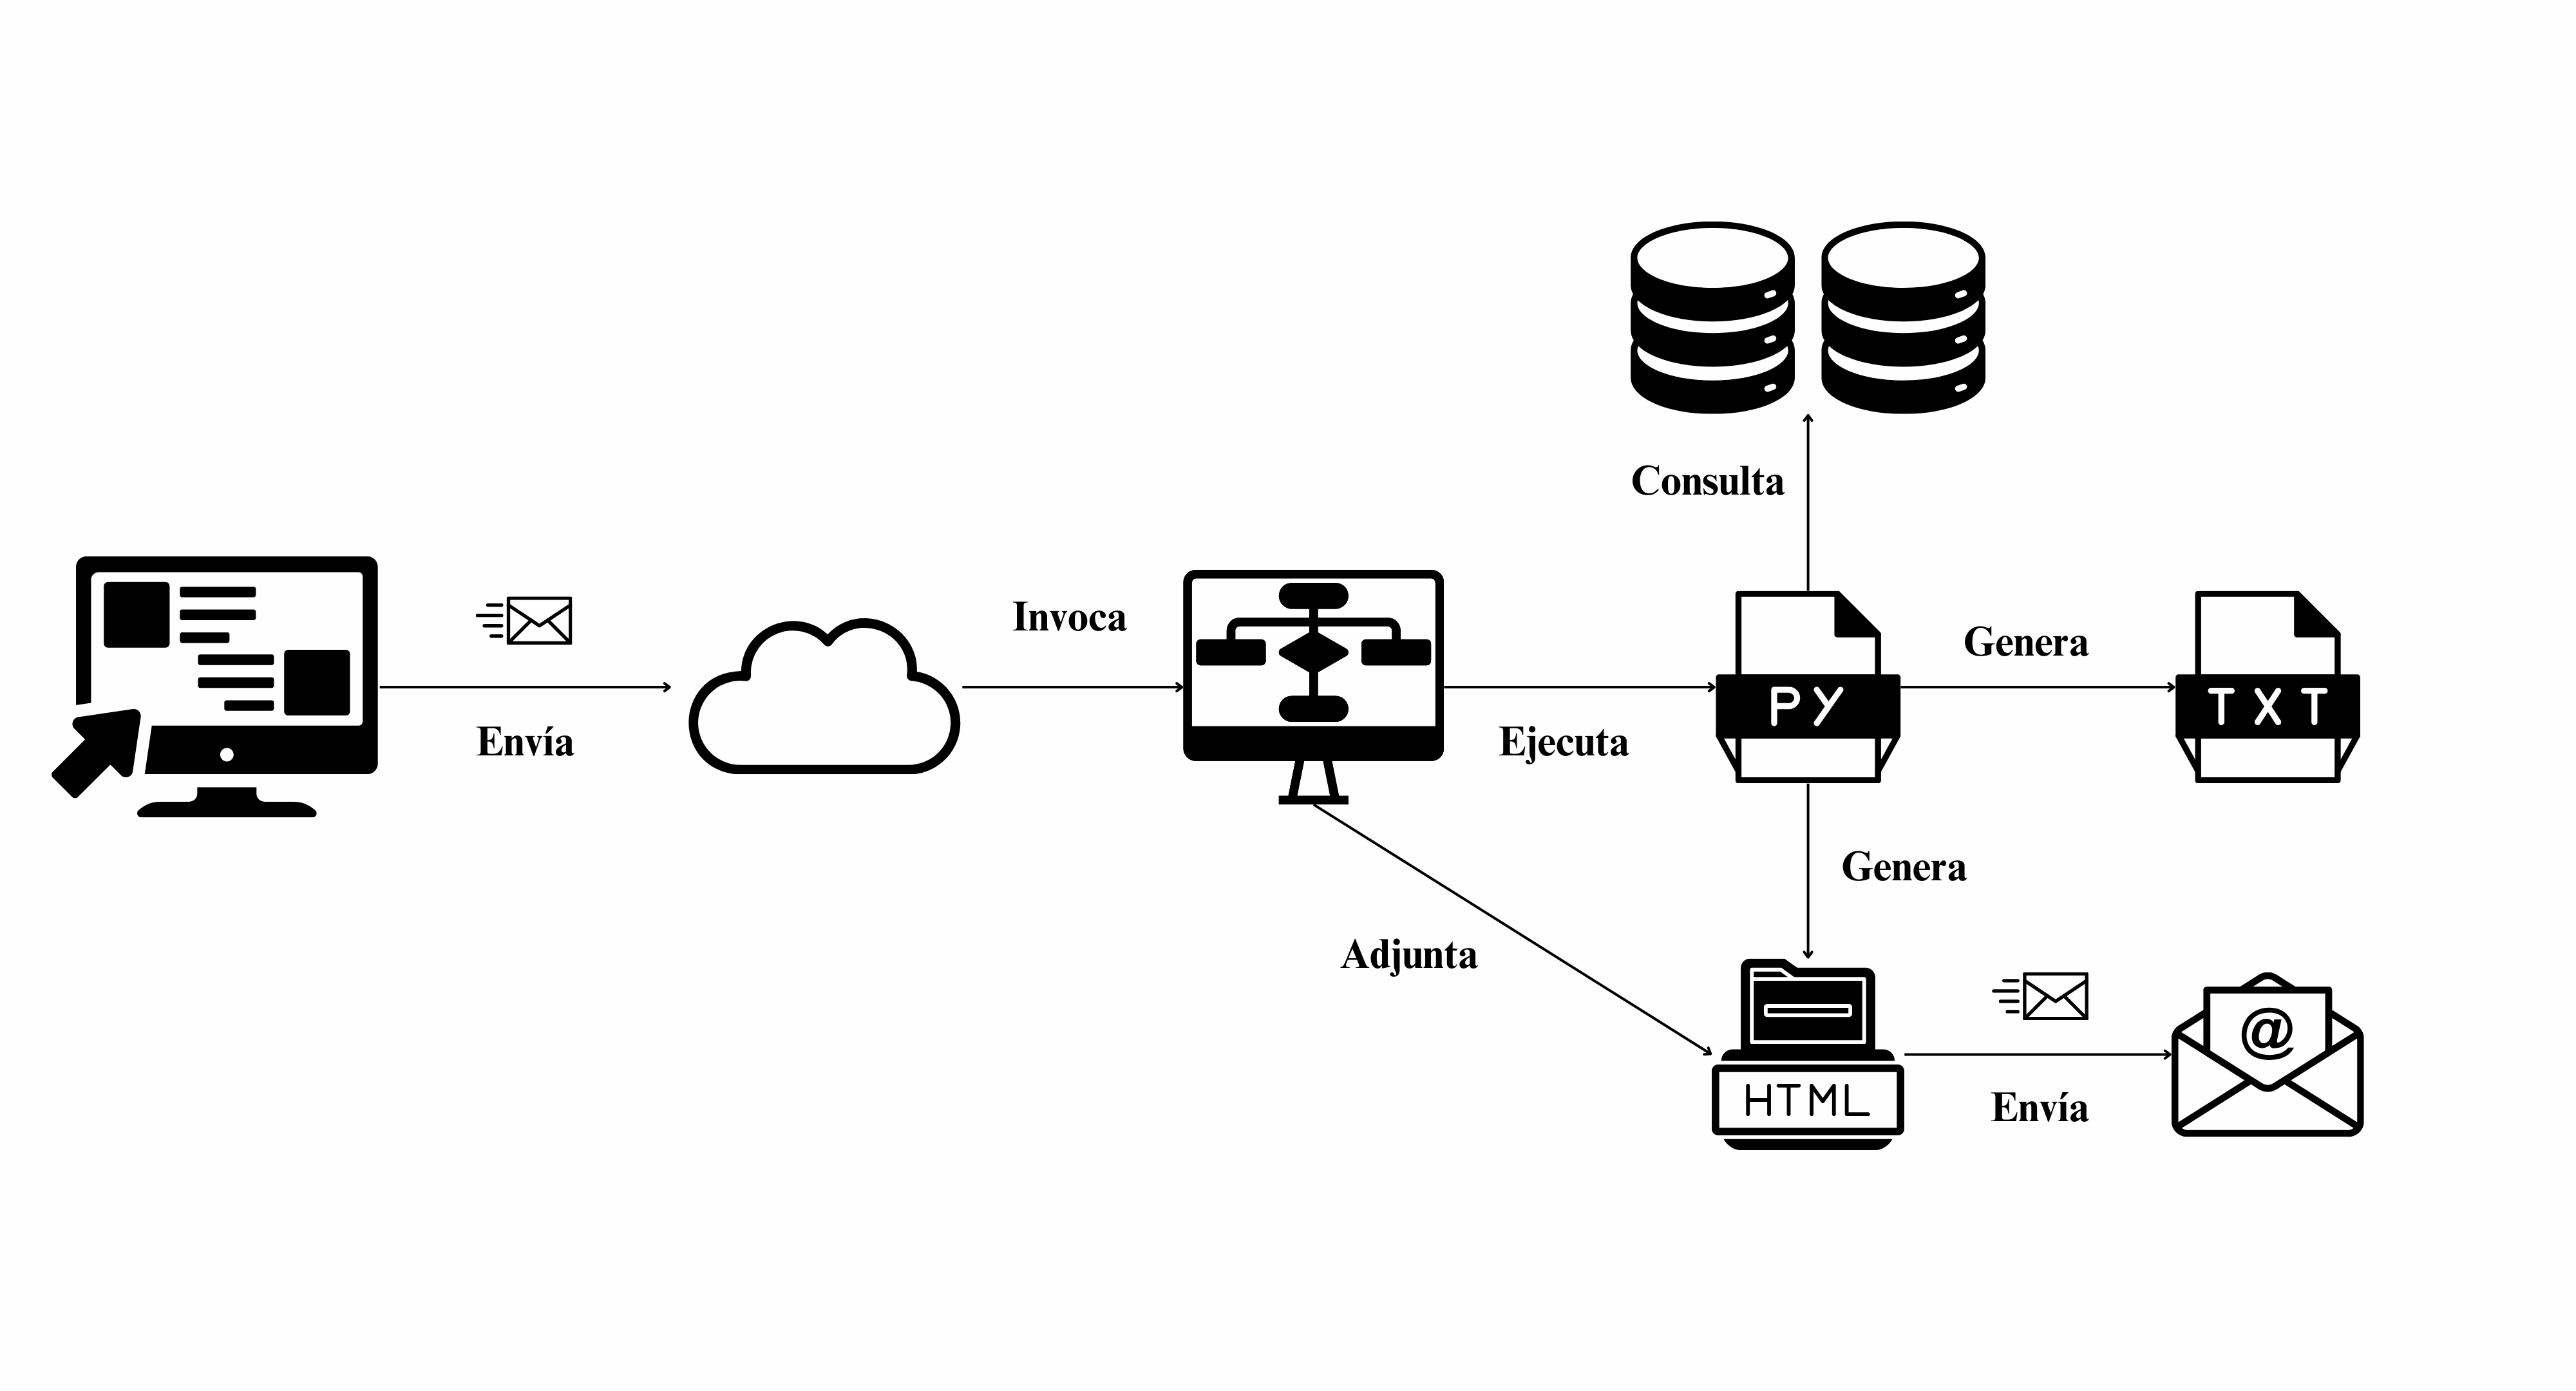
\includegraphics[width=0.7\textwidth]{Figs/ARQUITECTURA.png}
    \label{fig:Arquitectura}
    \\Nota: Arquitectura completa de la solución desarrollada. León, J. (2024). Diseño propio.
\end{figure}



\noindent Para el desarrollo de este trabajo se realizó una investigación y validación a fondo con el fin de garantizar la integración entre las herramientas y su correcto uso, teniendo en cuenta impedimentos a nivel empresarial, técnico y basándose en las reglas de negocio previamente socializadas con el usuario y su necesidad. Esta investigación da cabida a la integración del proyecto cuyo punto de partida es la lógica de la información, iniciando así con la construcción y diseño del Paquete Python.

\section{Paquete Python}

\noindent Inicialmente se tuvo planteado la creación de un Script de Python que llevara la lógica completa, sin embargo, en aras de la organización, captura de errores y buenas prácticas, se desarrolla un \textbf{Paquete Python} (\cite{Beazley2013, Lutz2013}). Se refiere a una colección o conjuntos de Scripts que están estructuralmente conectados. Algunos términos que permiten describir la estructura son:

\begin{itemize}
    \item \textbf{Proyecto Python:} Se refiere al conjunto de Scripts o módulos que, al trabajar integrados, conforman una aplicación o sistema. Puede incluir archivos de Python \texttt{.py} con archivos individuales encargados de otras funcionalidades, como archivos de configuración, conexión, documentación y otros recursos (\cite{Martelli2006}).

    \item \textbf{Módulo:} Cada Script \texttt{.py} es técnicamente hablando, un módulo en Python. Un módulo es cualquier archivo de código Python, que define clases, funciones y variables, y puede ser importado por otros scripts para su uso (\cite{Pilgrim2004}).

    \item \textbf{Paquete:} Un paquete en Python es una colección de módulos organizados en directorios, que incluyen el archivo \texttt{init.py} para que Python los trate como un paquete importable. Los paquetes permiten estructurar proyectos de manera que las funcionalidades estén bien organizadas (\cite{Beazley2009}).

    \item \textbf{Biblioteca (Library):} Se refiere a un conjunto de módulos o paquetes que proporcionan funcionalidades específicas y están diseñados para ser reutilizables en otros proyectos (\cite{VanRossum2001}).
\end{itemize}

\noindent Un paquete Python ofrece las siguientes ventajas sobre un Script monolítico:

\begin{enumerate}
    \item \textbf{Mantenibilidad}
    \begin{itemize}
        \item \textbf{Código más organizado:} Dividir la lógica en módulos hace que el código sea más fácil de entender y mantener. Cada módulo tiene una responsabilidad específica, lo que facilita realizar modificaciones o correcciones sin afectar otras partes del sistema (\cite{Lutz2013}).
        
        \item \textbf{Modularización:} Al tener diferentes funcionalidades separadas, es más sencillo localizar errores o añadir nuevas funcionalidades sin necesidad de revisar o modificar todo el código (\cite{Beazley2013}).
    \end{itemize}

    \item \textbf{Reutilización de código}
    \begin{itemize}
        \item \textbf{Modularidad:} Los módulos pueden reutilizarse en otros proyectos; solo se requiere exportación, evitando la duplicidad de código y esfuerzos (\cite{Pilgrim2004}).
    
        \item \textbf{Paquetes compartidos:} Los paquetes tienen la posibilidad de ser compartidos con otros desarrolladores o bien distribuirse públicamente, lo que facilita la creación de librerías utilizables (\cite{VanRossum2001}).
    \end{itemize}

    \item \textbf{Escalabilidad}
    \begin{itemize}
        \item \textbf{Facilidad de expansión:} A medida que el proyecto crece en tamaño y complejidad, es más fácil agregar nuevas funcionalidades creando nuevos módulos en lugar de aumentar la longitud de un único Script (\cite{Beazley2013}).
    
        \item \textbf{Evitar sobrecarga de funciones:} Con un solo Script, las funciones acaban por ser bastante largas y difíciles de gestionar, incluso llegando al punto de recrear funciones que ya estaban diseñadas (\cite{Lutz2013}).
    \end{itemize}

    \item \textbf{Pruebas y depuración}
    \begin{itemize}
        \item \textbf{Pruebas unitarias:} Es más sencillo probar individualmente cada módulo y sus funcionalidades en un paquete modulado (\cite{Pilgrim2004}).
    
        \item \textbf{Depuración sencilla:} Llegado el caso en que suceda un error, localizar el problema es mucho más sencillo en un sistema modular. Es posible depurar un módulo específicamente en lugar de todo el sistema (\cite{Lutz2013}).
    \end{itemize}
\end{enumerate}

\noindent Teniendo en cuenta la viabilidad de realizar la lógica del Script modularmente en un Paquete, se da por inicio la creación de cada uno de estos, cada módulo está ligado con el principal, cuyo módulo mantiene el flujo de trabajo principal. Es este quien llama a cada uno de los módulos consiguientes para procesar la información. (Ver Figura \ref{fig:EstructurePacketPython})


\begin{figure}[ht]
    \centering
    \captionof{figure}{ \\ \vspace{0.5cm} Gráfico de la estructura del Paquete Python.}
    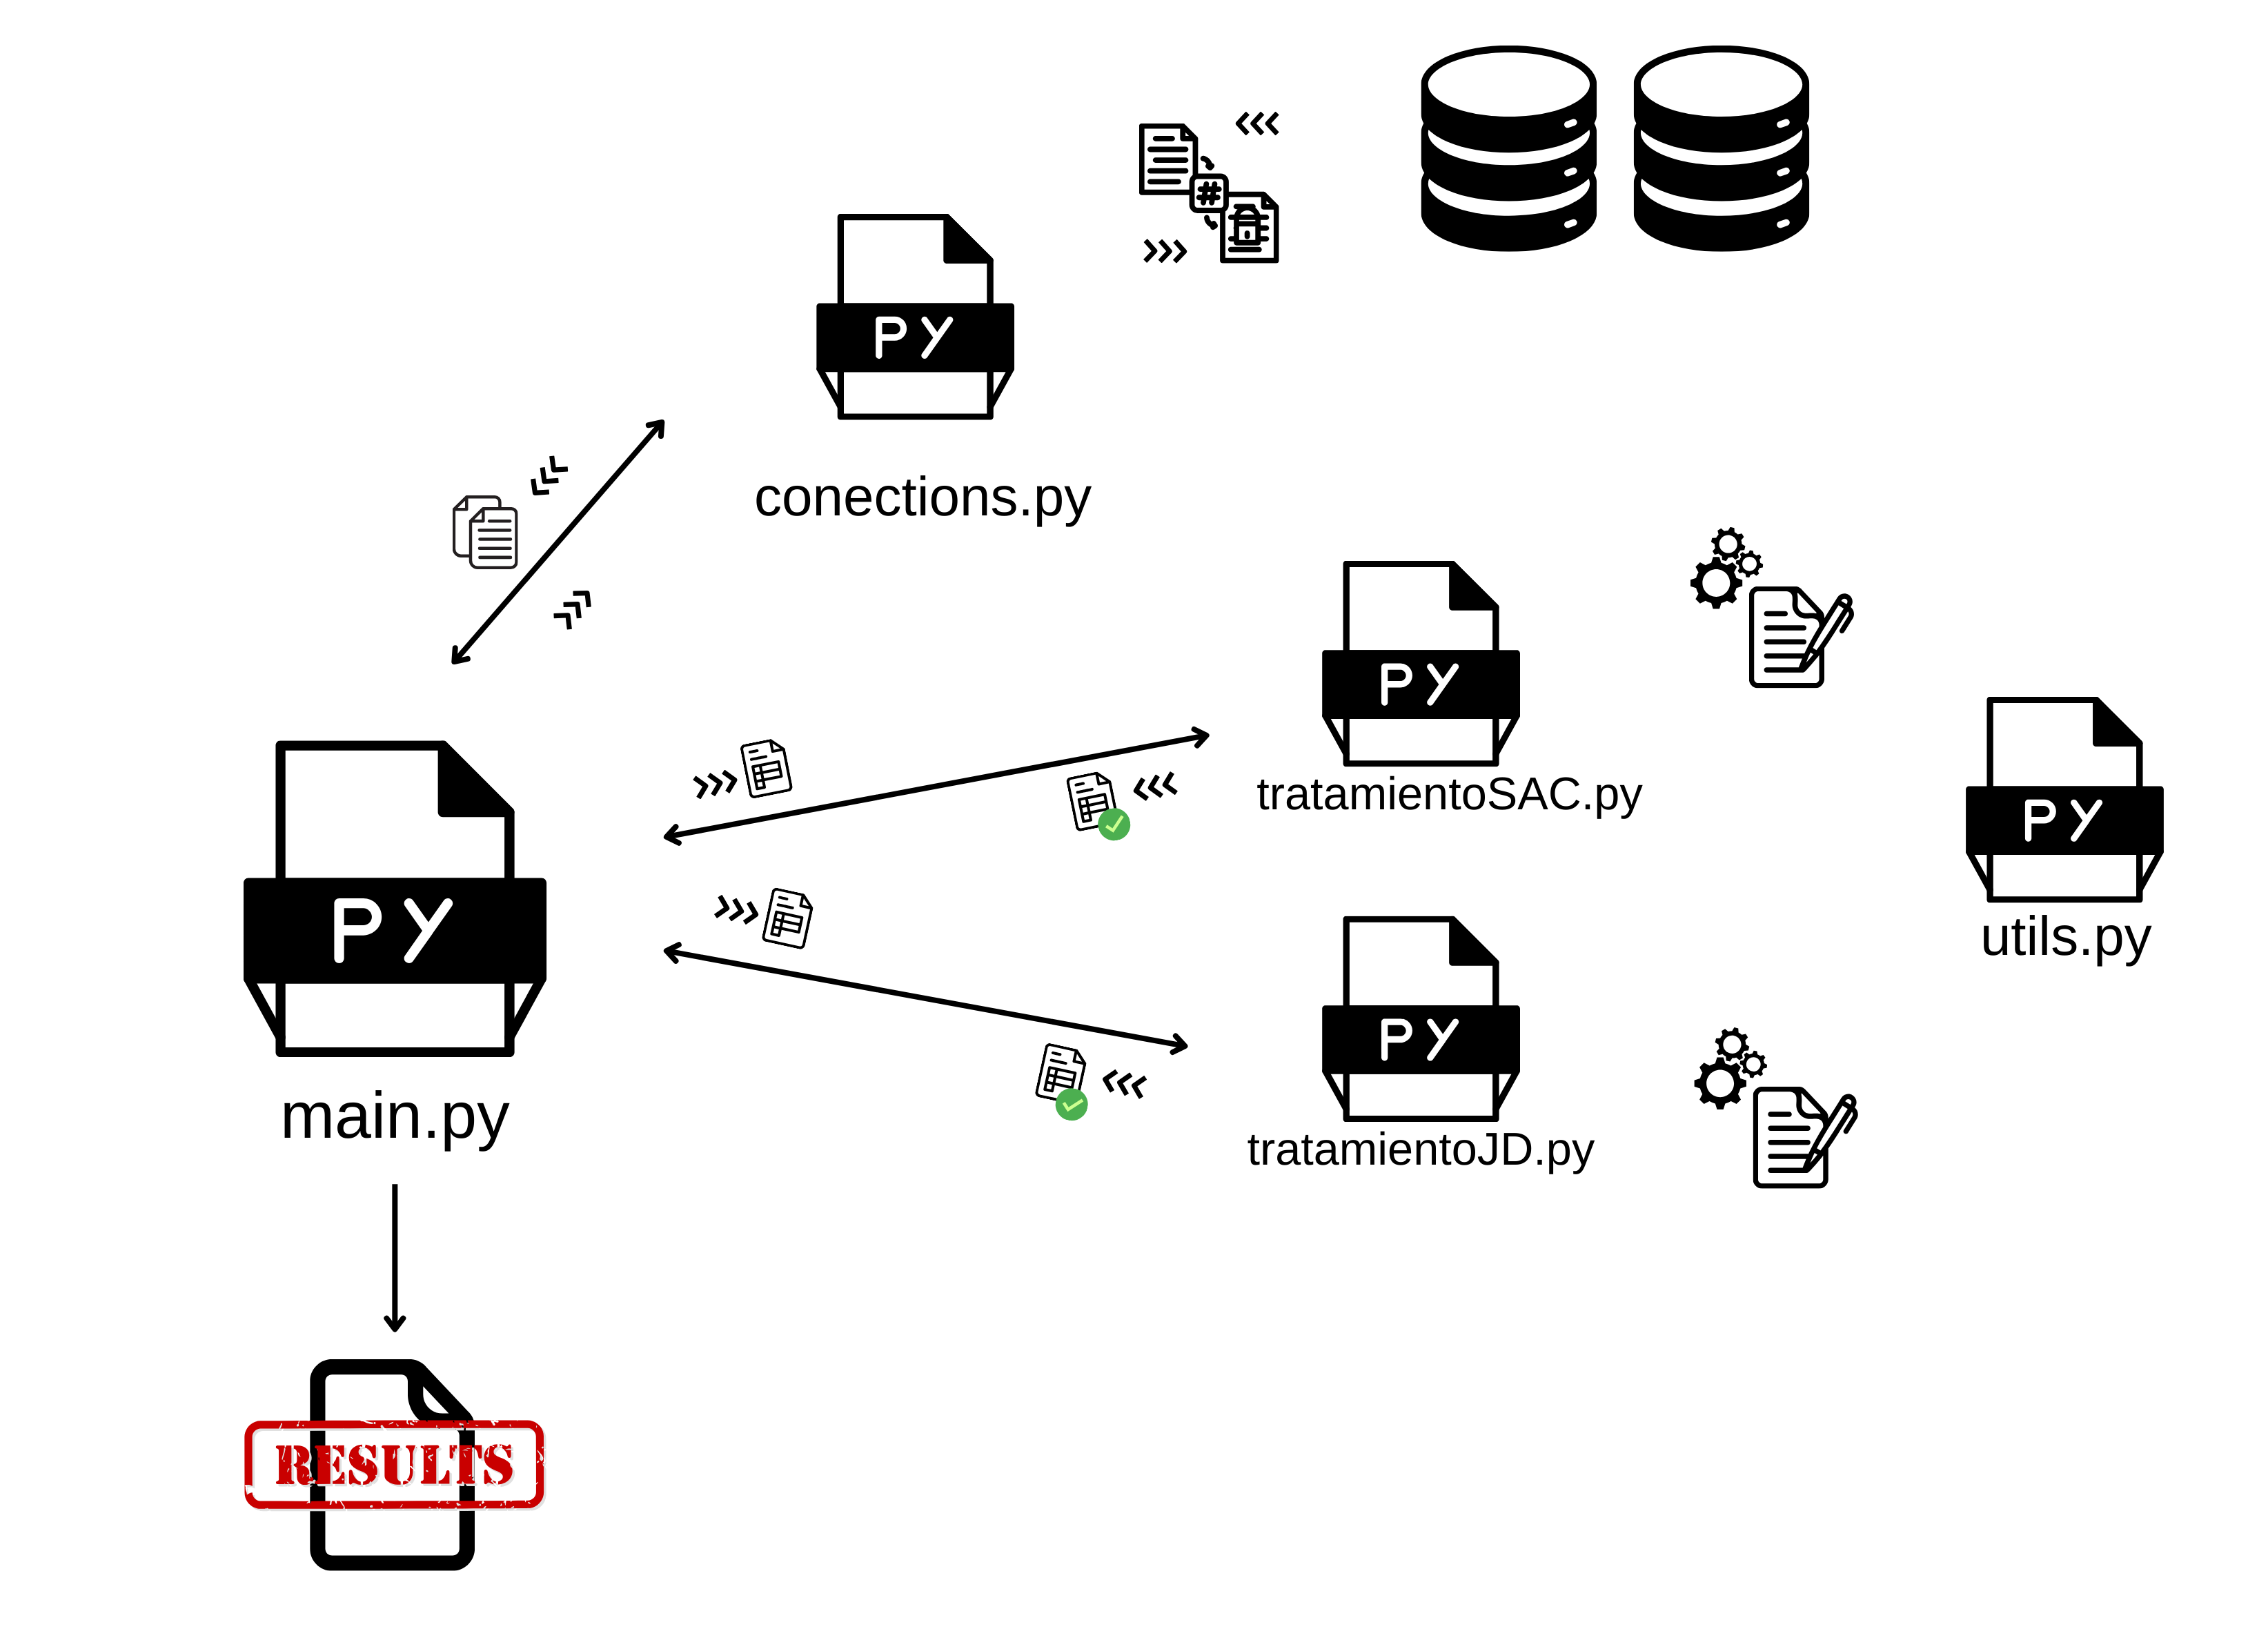
\includegraphics[width=0.7\textwidth]{Figs/Estructura Paquete Python.png}
    \label{fig:EstructurePacketPython}
    \\Nota: Gráfico estructural de la integración modular del paquete de Python. León, J. (2024). Diseño propio.
\end{figure}

\section{Automatización Robótica de Procesos}

\noindent Se desarrolla un flujo de trabajo con la lógica para ejecutar el Paquete Pytho, sin embargo, ¿cómo este flujo se va a disparar? Se propuso inicialmente que sea por medio de un correo electrónico vía Outlook que es de por si un conector de Microsoft Power Automate, el proceso de construcción de la lógica se divide en dos módulos de Automate, flujos de nube para el desencadenamiento de estos, ya que los flujos de escritorio no tienen trigger, y los correos se hace por medio de la nube de Microsoft, y por otro lado el flujo de escritorio que es el encargado de la ejecución directa en la línea de comandos del Paquete Python.


\section{Interfaz Gráfica de Usuario}

\noindent La interfaz fue creada en Microsoft Power Apps la cual consta de una sola pantalla, teniendo en cuenta que la interfaz es para efectos de generación de la lógica fuerte del proyecto, se decidió mantener pantallas emergente donde la lógica de visibilidad es basada en botones.

\begin{figure}[ht]
    \centering
    \captionof{figure}{ \\ \vspace{0.5cm} Pantalla inicial GUI. \textbf{Form CGN}.}
    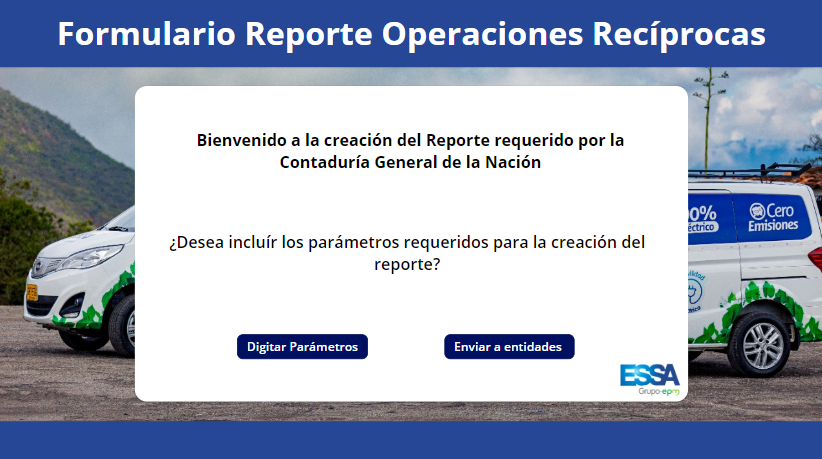
\includegraphics[width=0.45\textwidth]{Figs/Pantalla Inicial - APP.png}
    \label{fig:MainScreen}
    \\Nota: Visualización de la composición de la pantalla inicial de la interfaz gráfica. León, J. (2024). Diseño propio.
\end{figure}


\begin{figure}[ht]
    \centering
    \captionof{figure}{ \\ \vspace{0.5cm} Acción Botón "Digitar Parámetros". \textbf{Form CGN}.}
    \includegraphics[width=0.45\textwidth]{Figs/Action Digitar Parámetros Button - APP.png}
    \label{fig:ActionButtonDigitar}
    \\Nota: Acción que realiza el botón "Digitar Parámetros". León, J. (2024). Diseño propio.
\end{figure}

\begin{figure}[ht]
    \centering
    \captionof{figure}{ \\ \vspace{0.5cm} Pantalla de diligenciamiento de parámetros \textbf{Form CGN}.}
    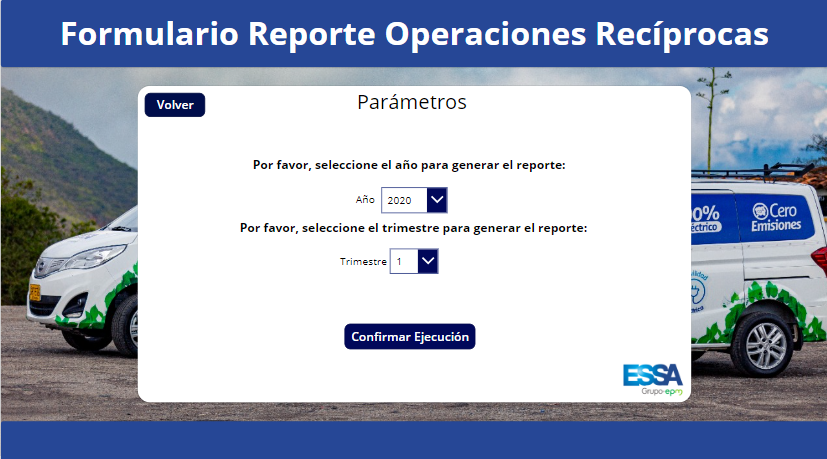
\includegraphics[width=0.45\textwidth]{Figs/Parametros - APP.png}
    \label{fig:DiligenciarScreen}
    \\Nota: Pantalla dedicada al diligenciamiento de parámetros para la generación del reporte. León, J. (2024). Diseño propio.
\end{figure}

\begin{figure}[ht]
    \centering
    \captionof{figure}{ \\ \vspace{0.5cm} Acción del botón de confirmar ejecución.\textbf{Form CGN}.}
    \includegraphics[width=0.45\textwidth]{Figs/Action Confirmar Ejecución Button - APP.png}
    \label{fig:ActionButtonConfirmar}
    \\Nota: Acción que realiza el botón "Confirmar Ejecución". León, J. (2024). Diseño propio.
\end{figure}

\begin{figure}[ht]
    \centering
    \captionof{figure}{ \\ \vspace{0.5cm} Pantalla emergente de re confirmación de generación. \textbf{Form CGN}.}
    \includegraphics[width=0.45\textwidth]{Figs/Reconfirmación - APP.png}
    \label{fig:ReconfirmarScreen}
    \\Nota: Pantalla emergente que resume los parámetros escogidos y re confirma la ejecución. León, J. (2024). Diseño propio.
\end{figure}

\begin{figure}[ht]
    \centering
    \captionof{figure}{ \\ \vspace{0.5cm} Acción del botón Generar Reporte.\textbf{Form CGN}.}
    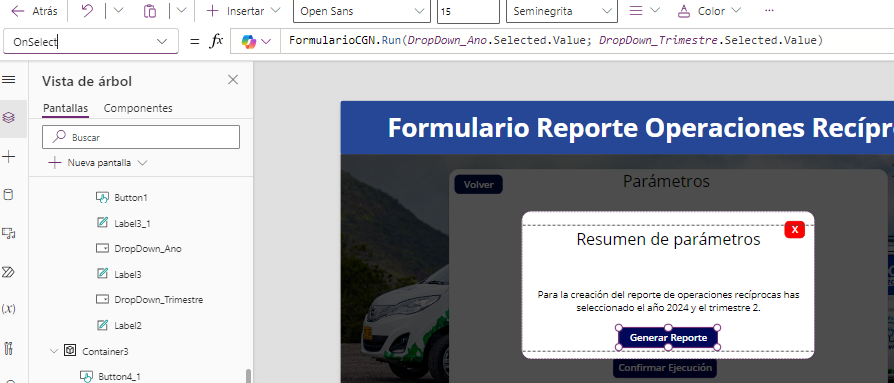
\includegraphics[width=0.5\textwidth]{Figs/Action Generar Reporte Button - APP.png}
    \label{fig:ActionGenerate}
    \\Nota: Acción que realiza el botón "Generar Reporte". León, J. (2024). Diseño propio.
\end{figure}


\begin{figure}[ht]
    \centering
    \captionof{figure}{ \\ \vspace{0.5cm} Flujo desencadenado por el botón "Generar Reporte". \textbf{Form CGN}.}
    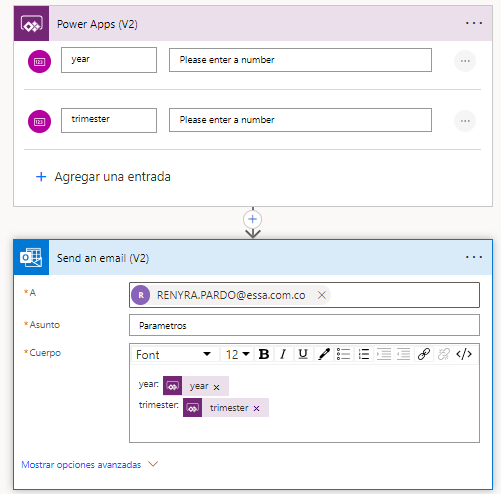
\includegraphics[width=0.5\textwidth]{Figs/Formulario CGN Flow - APP.png}
    \label{fig:FlowParams}
    \\Nota: Flujo cuyo trigger es el botón de la GUI de Power Apps, recibe parámetros y los envía por correo. León, J. (2024). Diseño propio.
\end{figure}


\begin{figure}[ht]
    \centering
    \captionof{figure}{ \\ \vspace{0.5cm} Acción del botón Envío a Entidades.\textbf{Form CGN}.}
    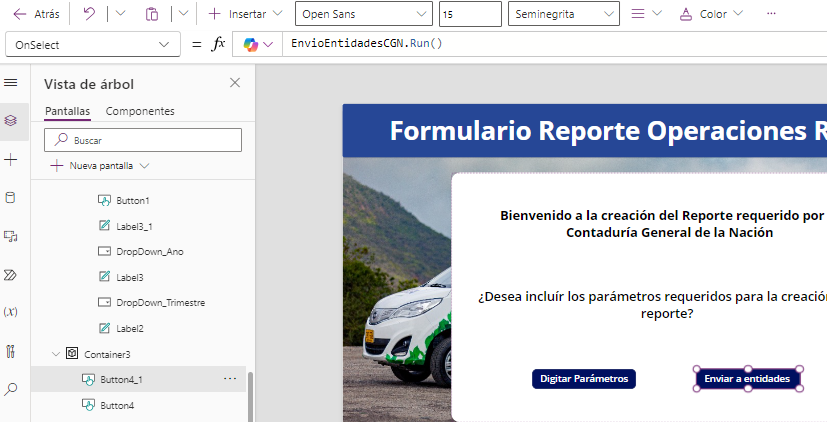
\includegraphics[width=0.45\textwidth]{Figs/Action Enviar a entidades - APP.png}
    \label{fig:ActionSendButton}
    \\Nota: Acción que realiza el botón "Envío a entidades". León, J. (2024). Diseño propio.
\end{figure}


\begin{figure}[ht]
    \centering
    \captionof{figure}{ \\ \vspace{0.5cm} Flujo desencadenado por el botón "Envío a entidades". \textbf{Form CGN}.}
    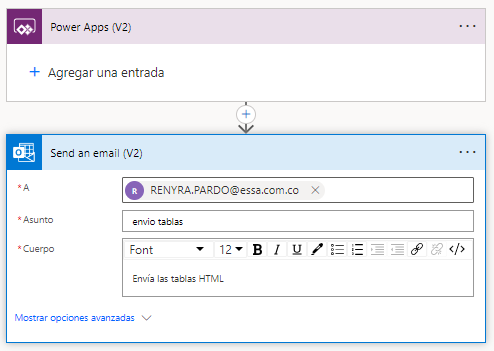
\includegraphics[width=0.4\textwidth]{Figs/Envio Entidades Flow - APP.png}
    \label{fig:FlowSend}
    \\Nota: Flujo cuyo trigger es el botón de la GUI de Power Apps y envía una señal de ejecución por correo. León, J. (2024). Diseño propio.
\end{figure}

\noindent Fue desarrollada con parametrización a la hora de elegir los parámetros de ejecución, usando dropbox en lugar de cajas de texto propensas a errores de digitación e incluso una doble confirmación de ejecución para evitar mala diligencia de parámetros.


\noindent Inicialmente se tiene una primera pantalla con dos botones, uno pretende guiar al usuario a la digitación de los parámetros, y el otro al envío de las tablas HTML vía correo a cada entidad. (Ver Figura \ref{fig:MainScreen})


\noindent La acción del botón \textbf{Digitar Parámetros}, es hacer visible eel grupo de componentes que desarrollan la siguiente pantalla de digitalización, cambiando el valor booleano de las variables de visualización de cada componente. (Ver Figuras \ref{fig:ActionButtonDigitar}, \ref{fig:DiligenciarScreen})

\noindent En la pantalla de diligenciamiento de parámetros se tienen dos componentes \textbf{DropBox} o \textbf{Caja Desplegable} que permite al usuario elegir el año y el trimestre para el que requiere la generación del reporte. 

\noindent Posterior a esta acción, el usuario confirma la efecución por medio del botón \textbf{Confirmar ejecución}, que manteniendo la lógica del anterior botón, hace visible una pantalla emergente que resumen los parámetros escogidos y re confirma la generación del reporte. Ver figuras (\ref{fig:ActionButtonConfirmar}, \ref{fig:ReconfirmarScreen})

\noindent Este botón de \textbf{Generar Reporte} tiene en su propiedad \textbf{OnSelect} la ejecucuón de un flujo de nube que tiene como parámetros los valores de las cajas desplegables, y las envía por correo a la cuenta técnica que contiene la solución. (Ver Figuras \ref{fig:ActionGenerate},\ref{fig:FlowParams})

\noindent Adicional a esto la acción y el flujo de envío de las tablas HTML, son generador por el botón \textbf{Envío a entidades}, cuya acción es desencadenar un flujo que envía una señal vía correo a la cuenta técnica que hospeda el flujo con tal lógica. (Ver Figuras \ref{fig:ActionSendButton},\ref{fig:FlowSend})


\newpage

\section{Implementación de seguridad}

\noindent La implementación de seguridad se realizó inicialmente en la encriptación de credenciales para realizar la conexión a las bases de datos, por medio de un módulo del paquete de python, presentado en sesiones anteriores, donde su realización es de la siguiente manera:


\noindent También se realizar implementación de seguridad en la conexión a las bases de datos, ya que la librería \texttt{Python-oracledb} la cual hace enlace mediante el protocolo SSL/TLS para el cifrado de las conexiones, por otro lado la organización maneja el uso de firewalls y VPN como seguridad en las conexiones.

\noindent Por otra parte la implementación de la seguridad en los servicios explicada en sesiones anteriores, se hace uso de esta implementación ortorgando permisos a los usuarios debido y manteniendo una gestión del flujo completo de la solución.


\section{Despliegue y Estabilización}

\noindent El despliegue de esta solución se realizó transfiriendo el Paquete Python al servidor donde se va a hospedar. Incluyendo requerimientos como la instalación de las librerías:

\begin{figure}[ht]
    \centering
    \captionof{figure}{ \\ \vspace{0.5cm} Componentes de la solución. \textbf{RPA\_ReporteCGN}.}
    \includegraphics[width=0.4\textwidth]{Figs/Objetos de la solución - RPA_ReporteCGN.png}
    \label{fig:ComponentSolution}
    \\Nota: Componentes integrados en la solución RPA\_ReporteCGN. León, J. (2024). Diseño propio.
\end{figure}

\begin{figure}[ht]
    \centering
    \captionof{figure}{ \\ \vspace{0.5cm} Exportación de la solución. \textbf{RPA\_ReporteCGN}.}
    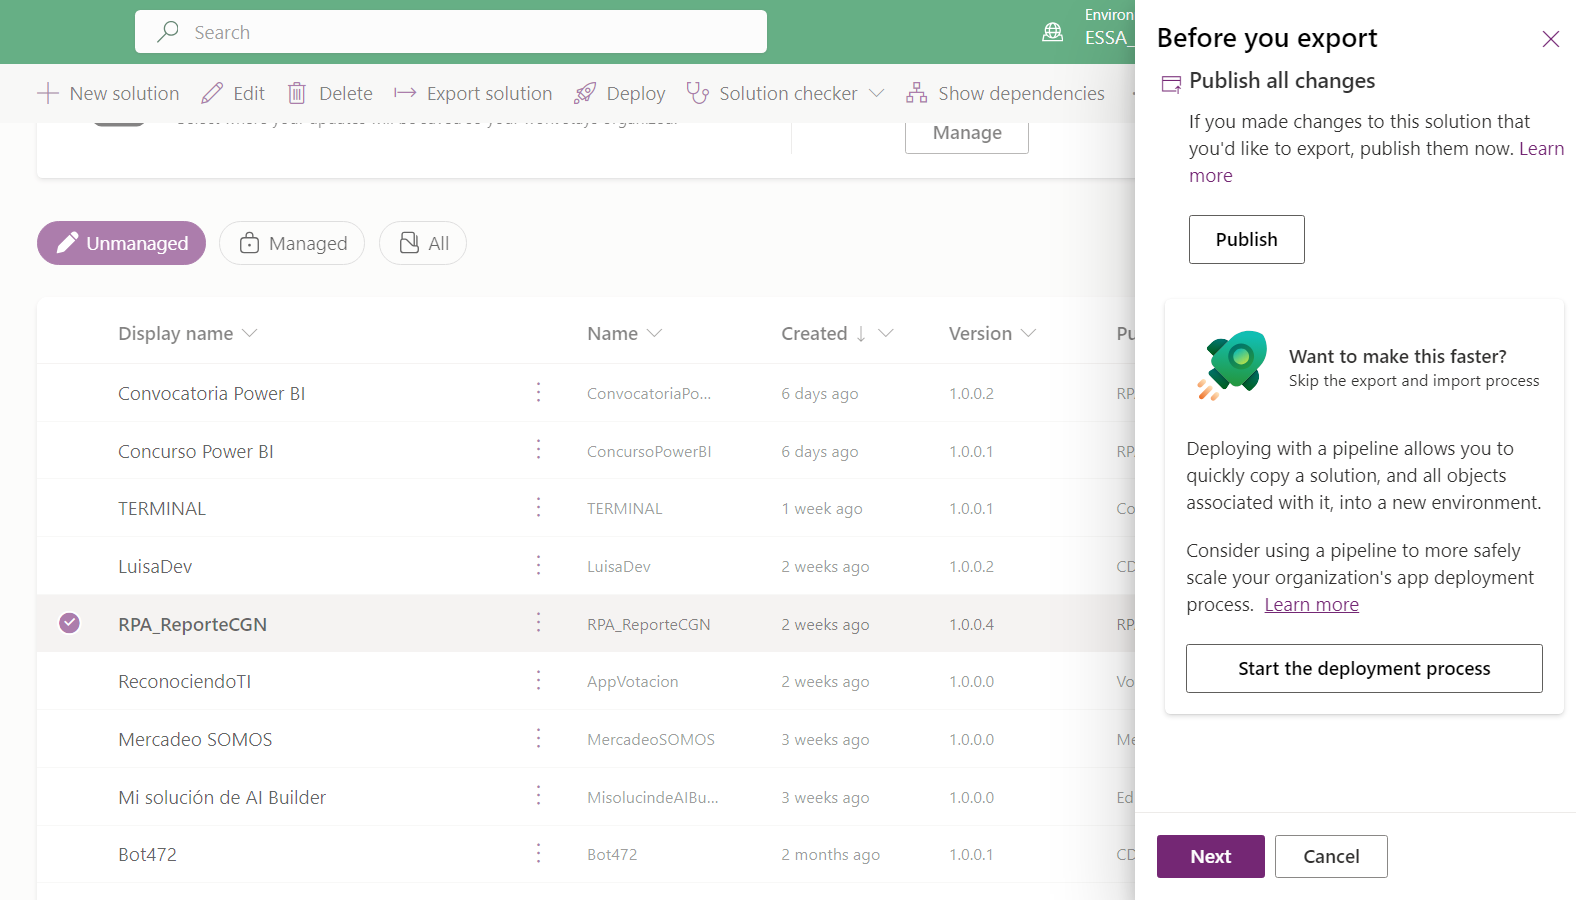
\includegraphics[width=0.4\textwidth]{Figs/Exportación Solución - RPA_ReporteCGN.png}
    \label{fig:ExportationSolution}
    \\Nota: Exportación de la solución RPA\_ReporteCGN en modo managed. León, J. (2024). Diseño propio.
\end{figure}

\begin{figure}[ht]
    \centering
    \captionof{figure}{ \\ \vspace{0.5cm} Paquete de la solución descargado. \textbf{RPA\_ReporteCGN}.}
    \includegraphics[width=0.4\textwidth]{Figs/Solución Exportada - RPA_ReporteCGN.png}
    \label{fig:SolutionExported}
    \\Nota: Descarga de la carpeta compartida de los componentes de la solución RPA\_ReporteCGN. León, J. (2024). Diseño propio.
\end{figure}

\begin{figure}[ht]
    \centering
    \captionof{figure}{ \\ \vspace{0.5cm} Importación de la solución. \textbf{RPA\_ReporteCGN}.}
    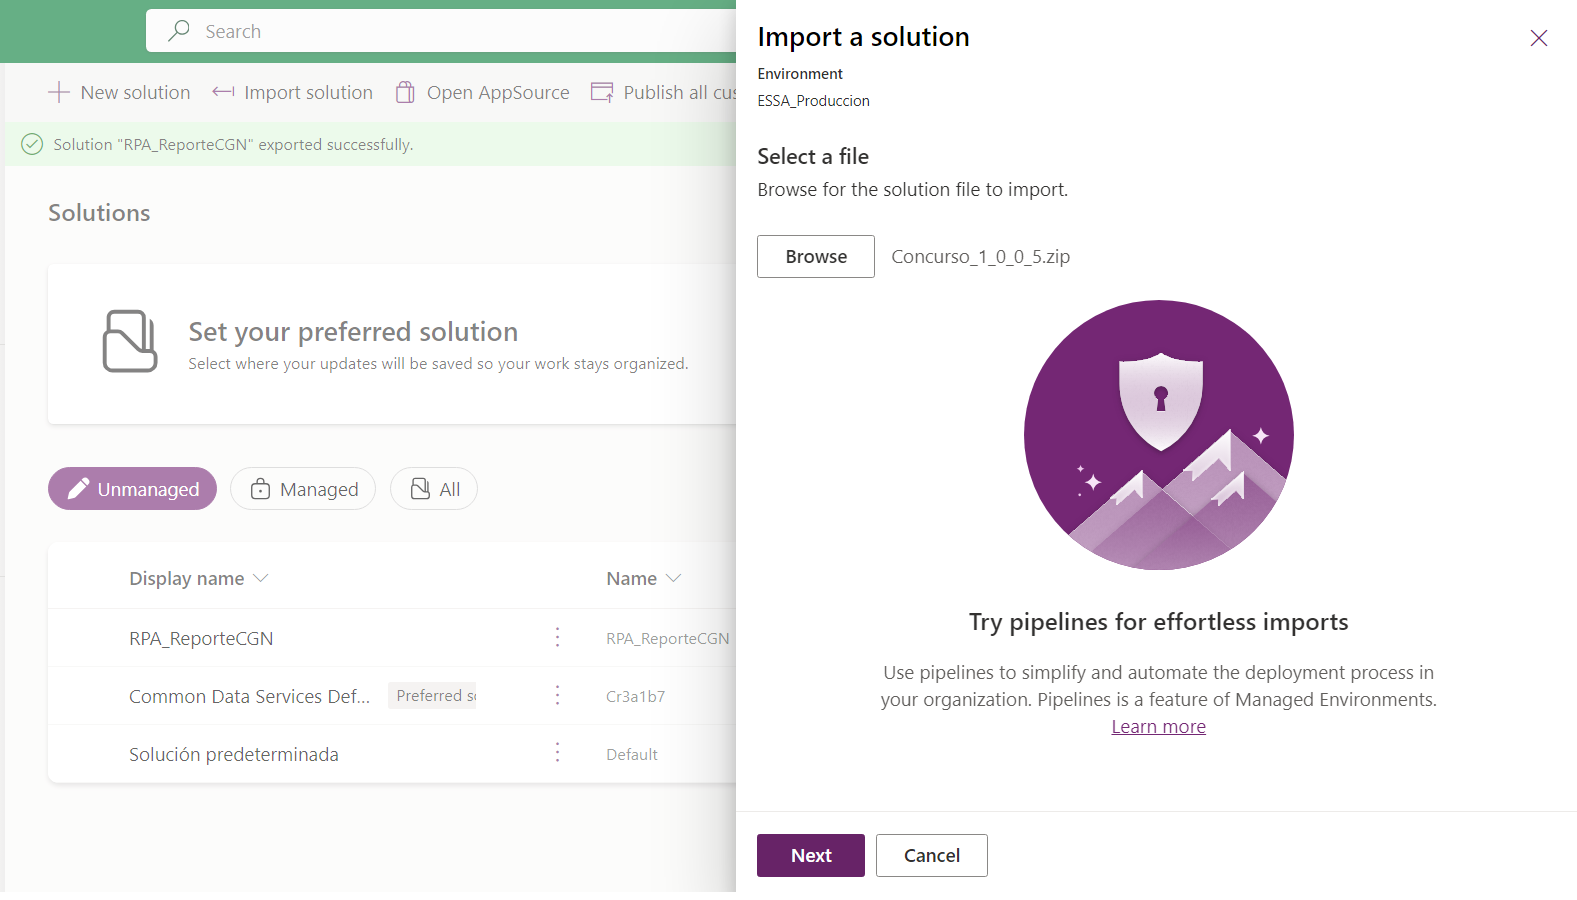
\includegraphics[width=0.55\textwidth]{Figs/Importación de la Solución - RPA_ReporteCGN.png}
    \label{fig:ImportationSolution}
    \\Nota: Importación de la solución RPA\_ReporteCGN en el entorno de producción. León, J. (2024). Diseño propio.
\end{figure}


\begin{figure}[ht]
    \centering
    \captionof{figure}{ \\ \vspace{0.5cm} Solución en producción. \textbf{RPA\_ReporteCGN}.}
    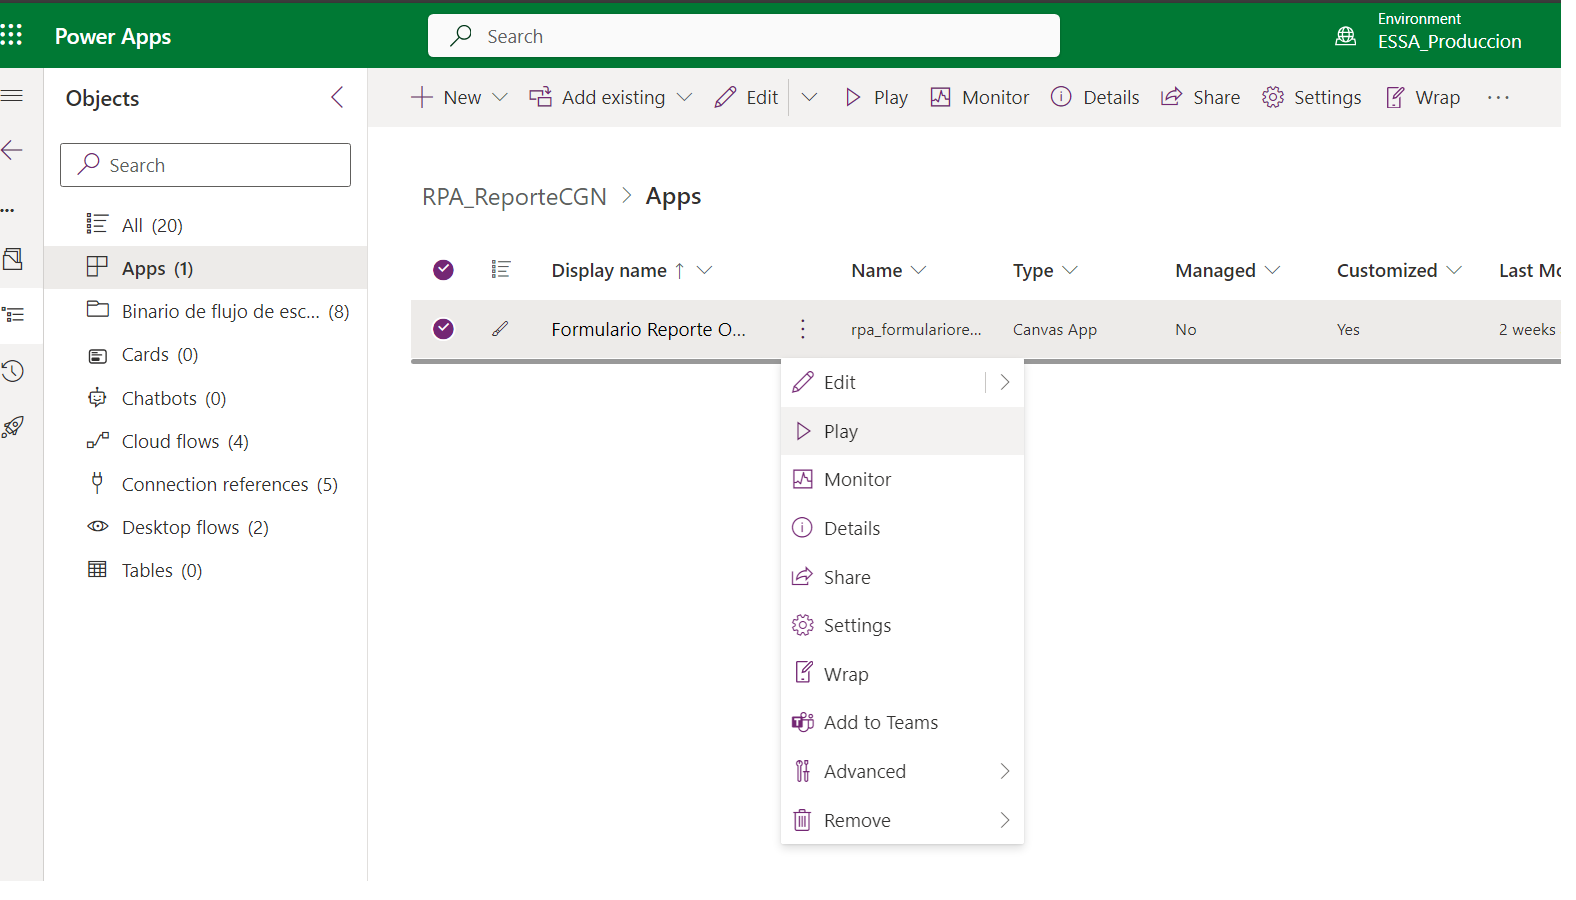
\includegraphics[width=0.4\textwidth]{Figs/Solución en Producción - RPA_ReporteCGN.png}
    \label{fig:SolutionInProduction}
    \\Nota: Solución RPA\_ReporteCGN ejecutada en producción. León, J. (2024). Diseño propio.
\end{figure}

\begin{itemize}
    \item \texttt{pandas}
    \item \texttt{Python-Oracledb}
    \item \texttt{json}
    \item \texttt{cryptography.Fernet}
    \item \texttt{Oracle Instant Client}
\end{itemize}

\noindent Ya que esta solución requiere de un lugar donde hospedar archivos, bien sea los resultantes, o los necesario para la ejecución, como lo son las conciliaciones y excepciones. Estos archivos se hospedan en una carpeta local compartida, que tiene acceso restringido, por ello tuvo que tramitarse los permisos únicamente del usuario del servidor donde está hospedada la solución, y el usuario que debe cargar los archivos u obtener los resultantes.

\noindent Se realiza despliegue a las conexión de las bases de datos, cambiando el ambiente al que se hace conexión, cambiando el host al que se apunta, el puerto y el sid o service name.


\noindent Para el despliegue de la parte de la solución desarrollada por herramientas de Microsoft, se debe crear una solución, integrando todos los elementos (Ver Figura \ref{fig:ComponentSolution}):

\begin{itemize}
    \item aplicación
    \item flujos de nube
    \item flujos de escritorio
    \item referencias de conexión
    \item conectores
\end{itemize}



\noindent Teniendo la solución creada en el entorno de desarrollo, se procede a exportarla en modo \textbf{Managed} por buenas prácticas. (Ver Figura \ref{fig:ExportationSolution})




\noindent Esta solución exporta todos los componentes en una carpeta comprimida (\texttt{.zip}). (Ver Figura \ref{fig:ExportationSolution})



\noindent Posterior a la descarga se realiza el cambio de entorno a producción y se importa la solución (Ver Figura \ref{fig:ImportationSolution})




\noindent Finalmente se ejecuta la solución en producción (Ver Figura \ref{fig:SolutionInProduction}



\section{Pruebas}

\begin{figure}[ht]
    \centering
    \captionof{figure}{ \\ \vspace{0.5cm} Pruebas flujo de nube que desencadena la solución}
    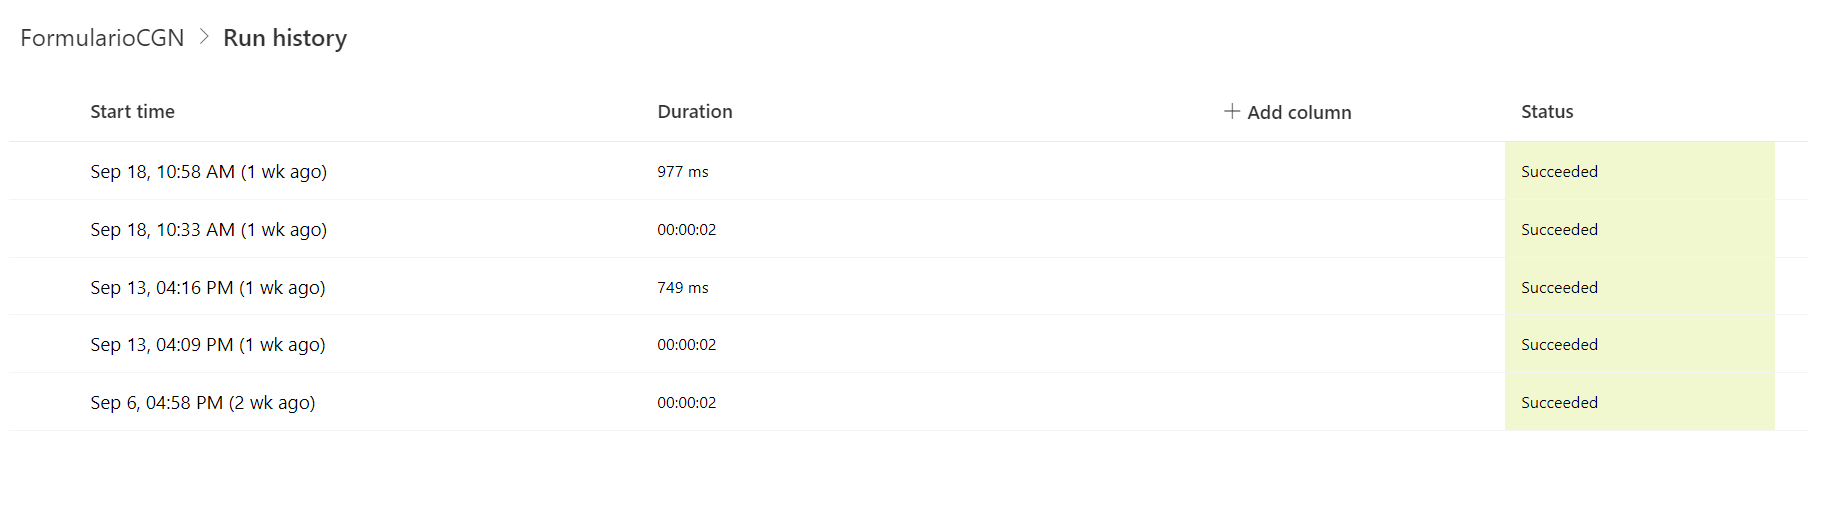
\includegraphics[width=0.4\textwidth]{Figs/Pruebas - FormulacioCGN.png}
    \label{fig:FlowAPPPTest}
    \\Nota: Prueba de las ejecuciones por parte del flujo desencadenado por la interfaz gráfica y desencadenador del flujo que invoca el flujo de escritorio. León, J. (2024). Diseño propio.
\end{figure}

\begin{figure}[ht]
    \centering
    \captionof{figure}{ \\ \vspace{0.5cm} Pruebas flujo de nube hospedado en cuenta técnica}
    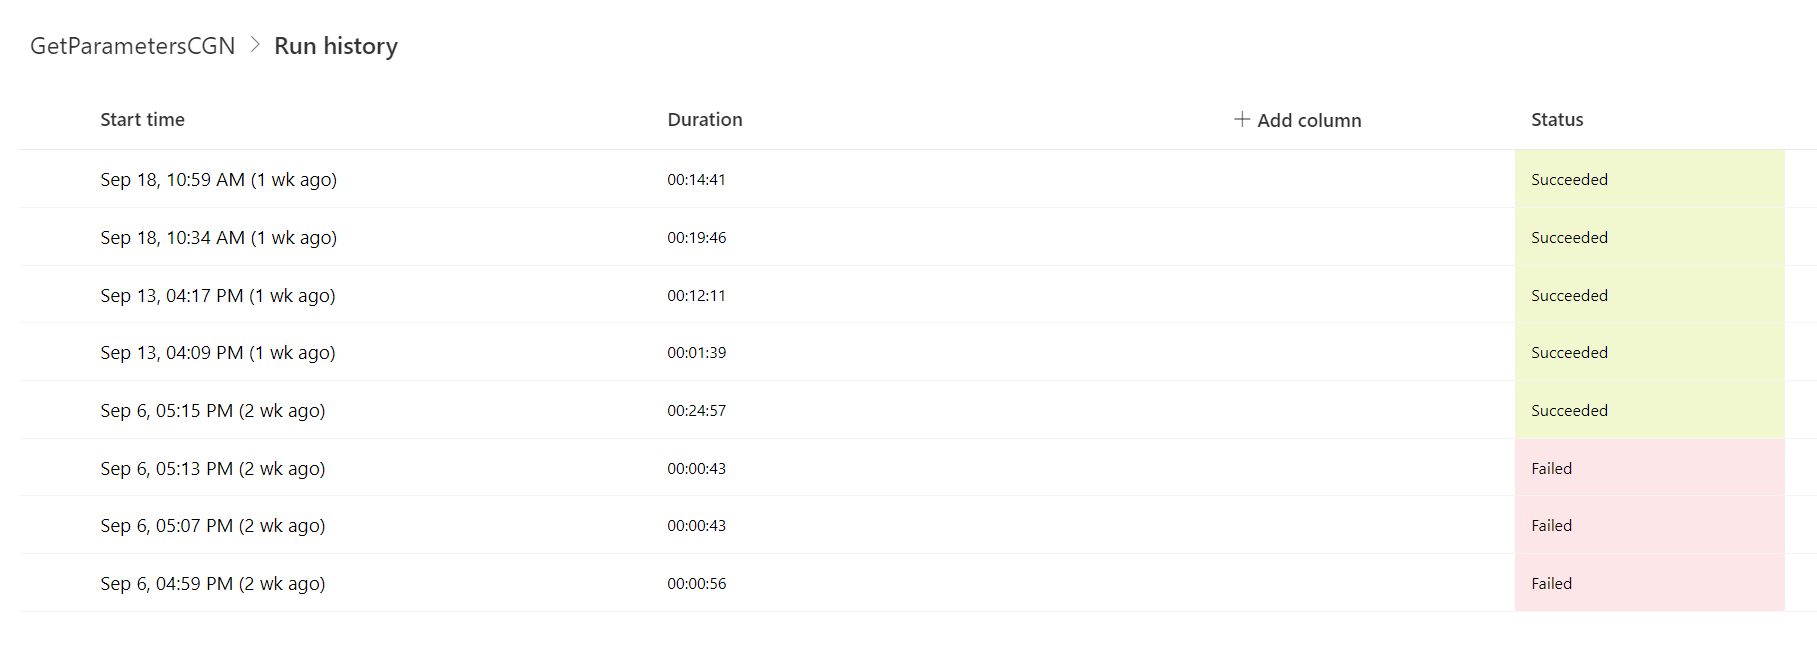
\includegraphics[width=0.4\textwidth]{Figs/Pruebas - GetParametersCGN.png}
    \label{fig:FlowCloudTest}
    \\Nota: Prueba de ejecución del flujo que recibe los parámetros e invoca el flujo de escritorio. León, J. (2024). Diseño propio.
\end{figure}  

\begin{figure}[ht]
    \centering
    \captionof{figure}{ \\ \vspace{0.5cm} Pruebas flujo de escritorio}
    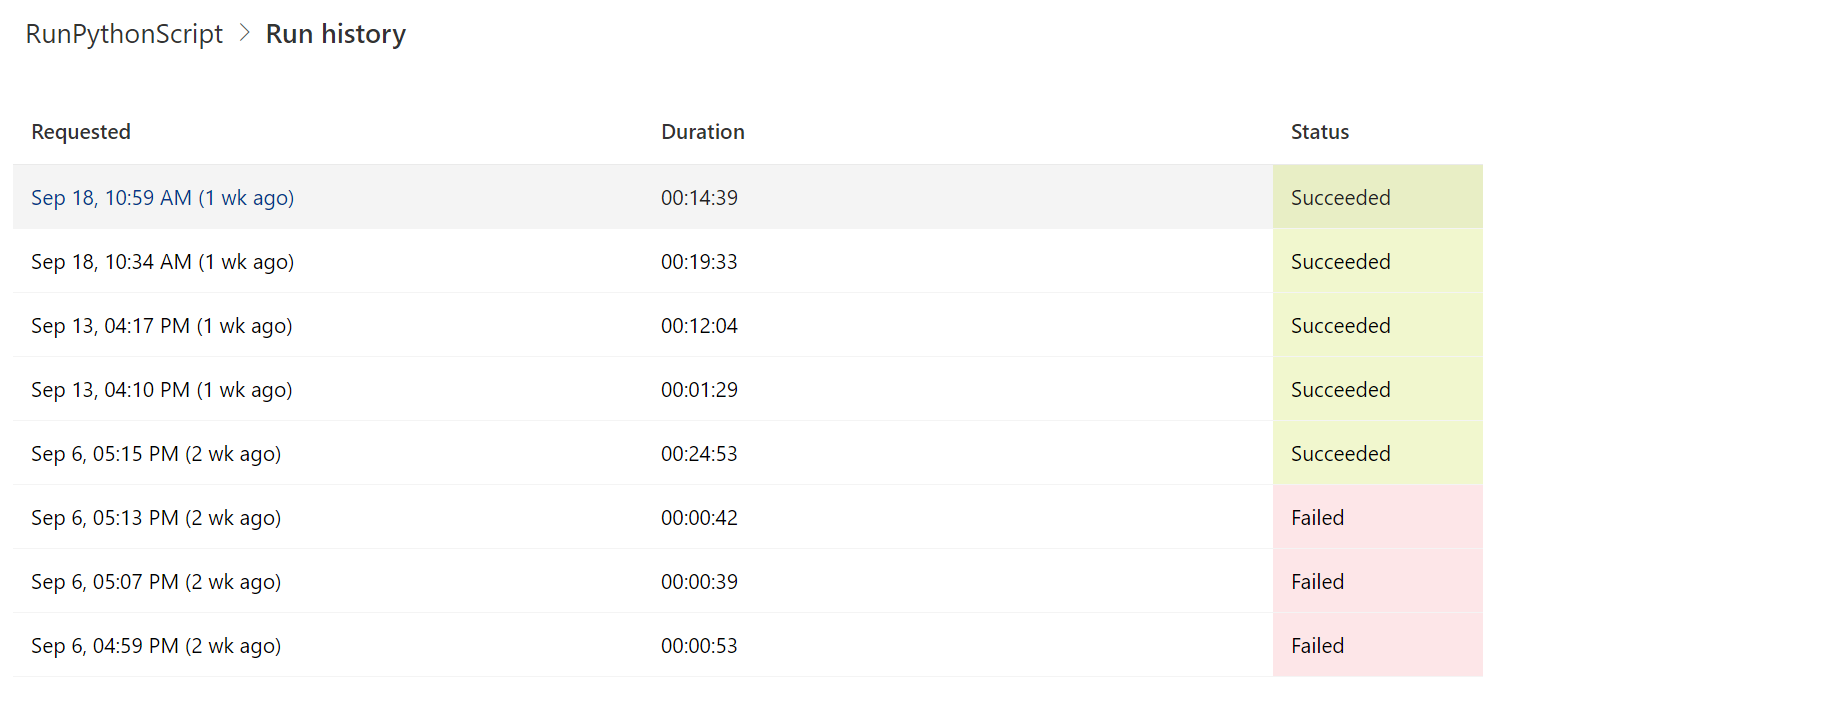
\includegraphics[width=0.4\textwidth]{Figs/Pruebas - RunPythonScript.png}
    \label{fig:FlowDesktopTest}
    \\Nota: Prueba de ejecución del flujo de escritorio que ejecuta el Paquete Python. León, J. (2024). Diseño propio.
\end{figure} 

\begin{figure}[ht]
    \centering
    \captionof{figure}{ \\ \vspace{0.5cm} Verificación reportes ejecutados}
    \includegraphics[width=0.4\textwidth]{Figs/Creación de reportes 1 y 2 trimeste - PRUEBAS.png}
    \label{fig:ReportInPath}
    \\Nota: Verificación de la creación del reporte en la ruta específica. León, J. (2024). Diseño propio.
\end{figure}   

\begin{figure}[ht]
    \centering
    \captionof{figure}{ \\ \vspace{0.5cm} Verificación reporte resultante}
    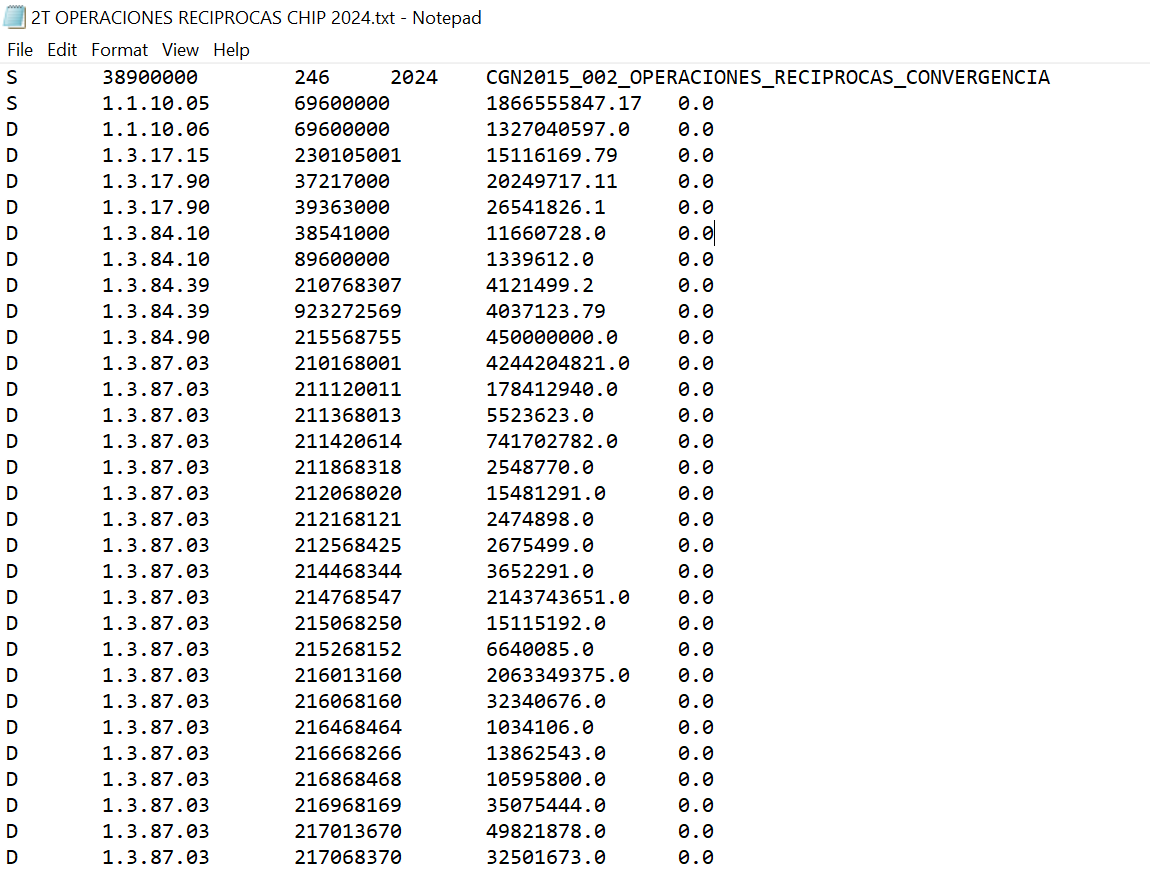
\includegraphics[width=0.4\textwidth]{Figs/reporte segundo trimestre.png}
    \label{fig:ReportTest}
    \\Nota: Verificación del formato del reporte y los valores. León, J. (2024). Diseño propio.
\end{figure}   



\noindent Se realizaron pruebas desde el punto más bajo de la solución (el paquete Python), hasta la solución en conjunto, desde la interfaz gráfica para el reporte del primer y segundo trimestre del presente año.



\begin{enumerate}
    \item Se ejecutan los parámetros desde la aplicación y se probaron las ejecuciones del flujo desecadenador que enviará los parámetros vía correo (Ver Figura \ref{fig:FlowAPPPTest})

    \item Con la ejecución del flujo, se estudia la ejecución del flujo que recibe los parámetros y ejecuta el flujo de escritorio a cargo del Paquete Python. (Ver Figura \ref{fig:FlowCloudTest})

   

    \item Ahora bien, teniendo pruebas se revisan las ejecuciones del flujo de escritorio que ejecuta el Paquete Python (Ver Figura \ref{fig:FlowDesktopTest})

    \item Se hacen verificaciones de la creación del reporte y se verifican sus valores los cuales coinciden, ya que se hace comparativa con los reportes ya realizados (Ver Figuras \ref{fig:ReportInPath},\ref{fig:ReportTest})

         
    \item Para el canal de envío del detalle (tablas HTML) a cada entidad se realiza de la misma manera, y fue exitoso el envío (Ver Figura \ref{fig:HTMLSend})
\end{enumerate}


\noindent Finalmente con cada ejecución se puede hacer una proyección de las ejecuciones y una comparativa referente al gatos previo a la implementación de la automatización. Los resultados de ejecución tienen un promedio de 20 minutos, esta ejecución es necesaria únicamente 4 veces al año, ya que su reporte se maneja con frecuencia trimestral. (Ver Figura \ref{fig:ConvsSinAutomatizacion})



% ------------------------------------------------------------------------


\newpage
\chapter{Conclusiones}


\noindent La integración de Python en entornos de Microsoft ha demostrado ser una solución eficiente y adaptable para la automatización de procesos complejos. Su capacidad para manejar grandes volúmenes de datos, junto con su amplia gama de bibliotecas especializadas como Pandas, ha facilitado el tratamiento y análisis de datos que, de otro modo, serían costosos y difíciles de gestionar utilizando únicamente herramientas nativas de Microsoft. La facilidad de integración con bases de datos permite realizar operaciones de manera rápida y eficaz, optimizando significativamente el tiempo de procesamiento de datos.

\noindent Como se muestra en la Figura \ref{fig:ConvsSinAutomatizacion} (a), el tratamiento manual de datos, que tradicionalmente llevaba alrededor de 540 horas al año, ha sido reducido en un 99.7\% mediante la automatización, disminuyendo el tiempo operativo a solo 80 minutos al año (Figura \ref{fig:ConvsSinAutomatizacion} (b)). Este ahorro de tiempo implica una liberación considerable de recursos humanos y tecnológicos, que ahora pueden ser reorientados hacia actividades de mayor valor añadido para la empresa, impulsando la productividad y la eficiencia operativa. Además, este enfoque refuerza la escalabilidad y flexibilidad de las soluciones basadas en Python en entornos corporativos, abriendo nuevas oportunidades para la mejora continua en la gestión de datos y la automatización de tareas.



\begin{figure}[ht]
    \centering
    \captionof{figure}{ \\ \vspace{0.5cm} Correo con detalle enviado.}
    \includegraphics[width=0.4\textwidth]{Figs/Tabla HTML envío correo.png}
    \label{fig:HTMLSend}
    \\Nota: Correo de llegada enviado por la cuenta técnica con la tabla HTML, exito de ejecución. León, J. (2024). Diseño propio.
\end{figure} 



% ------------------------------------------------------------------------

\newpage

\section{Trabajo Futuro}

\noindent A futuro, la automatización de procesos contables en la Electrificadora de Santander S.A. (ESSA) podría beneficiarse de la integración de Inteligencia Artificial (IA) y Machine Learning (ML), lo que permitiría que los bots adaptaran su comportamiento a cambios inesperados en los datos o procesos, mejorando la toma de decisiones y evolucionando hacia la Automatización de Procesos Inteligentes (IPA). Asimismo, la incorporación de tecnologías de Procesamiento de Lenguaje Natural (NLP) facilitaría la interpretación de información no estructurada, reduciendo la intervención humana.

\noindent Otra área de mejora es la seguridad de los datos. Aunque ya se emplean herramientas como Azure Key Vault, el uso de criptografía homomórfica permitiría procesar datos cifrados sin necesidad de desencriptarlos, aumentando así la protección de la información sensible. Además, la metodología desarrollada puede extenderse a otros departamentos de la empresa, como recursos humanos o finanzas, optimizando la eficiencia en varias áreas.

\noindent Finalmente, explorar otras plataformas de bajo código como Appsmith o Retool ofrecería mayor flexibilidad en los flujos de trabajo, y un análisis del impacto en la sostenibilidad podría alinear estos esfuerzos de automatización con los objetivos medioambientales de la empresa.





% ------------------------------------------------------------------------


% ------------------------------------------------------------------------
% Bibliografía
% ------------------------------------------------------------------------

\newpage

%\addcontentsline{toc}{chapter}{Referencias Bibliográficas}\newpage
%\bibliographystyle{apalike}
%\bibliography{biblio}
\addcontentsline{toc}{chapter}{Referencias Bibliográficas}

\printbibliography



\nocite{poniszewska-maranda, burns-kubernetes, torres-bosch-microservicios, armstrong2015,kubevirtio, docker2023, kubelet-doc, namespace-article}
% ------------------------------------------------------------------------
% Anexos


% ------------------------------------------------------------------------

% ------------------------------------------------------------------------
\end{document}                                          % Fin de documento
% ------------------------------------------------------------------------ 
